\subsection{Kalman Filter Extensions (Non-linear Kalman Filters)}


\begin{frame}
   \frametitle{Kalman Filter Extensions (Non-linear Kalman Filters)}
		
		\textbf{Objectives:} Since most real-life systems are non-linear, non-linear Kalman Filter design is essential 

            \textbf{Approach:}
		\begin{itemize}
            \item For non-linear systems handling, the \textit{Linear Approximation} techniques are applied
			\item Mathematical derivation and examples of the most common non-linear filters, designed based on \textit{Linear Approximation}:
            \begin{itemize}
                \item \textcolor{blue}{Extended Kalman Filter (EKF):} The EKF performs \textbf{analytic linearization} of the model at each point in time. EKF is the most common non-linear Kalman Filter.
                \item \textcolor{blue}{Unscented Kalman Filter (UKF) or Sigma-point Kalman Filter (SPKF):} The UKF performs \textbf{statistical linearization} of the model at each point in time.
            \end{itemize}
		\end{itemize}
  \textbf{Facts:} 
  \begin{itemize}
      \item While the standard Linear Kalman Filter (LKF) is an \textit{optimal filter} since we minimize the estimate uncertainty, all Kalman Filter modifications for non-linear systems are \textit{sub-optimal} since we use approximated models.
  \end{itemize}
\end{frame}




\begin{frame}
   \frametitle{An Early Implementation}
   
   		\begin{columns}
			\column{0.6\textwidth}
            *In fact, Kalman’s paper had not attracted much attention until Stanley Schmidt at the NASA Ames Research Center in Mountain View, California, recognized that it could be applied to the satellite and rocket-tracking problems just gaining prominence because of President Kennedy’s challenge to land a man on the moon. Schmidt made two important contributions to the success of Kalman’s ideas: 
            \begin{enumerate}
                \item He broke up the equations into the two steps of time updates and measurement updates, important if the data did not come in a steady stream, and
                \item Because the dynamics were nonlinear, he applied Kalman’s equations to linearized models, leading to the first of a family of what are known now as extended Kalman filters (EKF).
            \end{enumerate}
			
			\column{0.4\textwidth}
		
			\begin{figure}
				\centering
					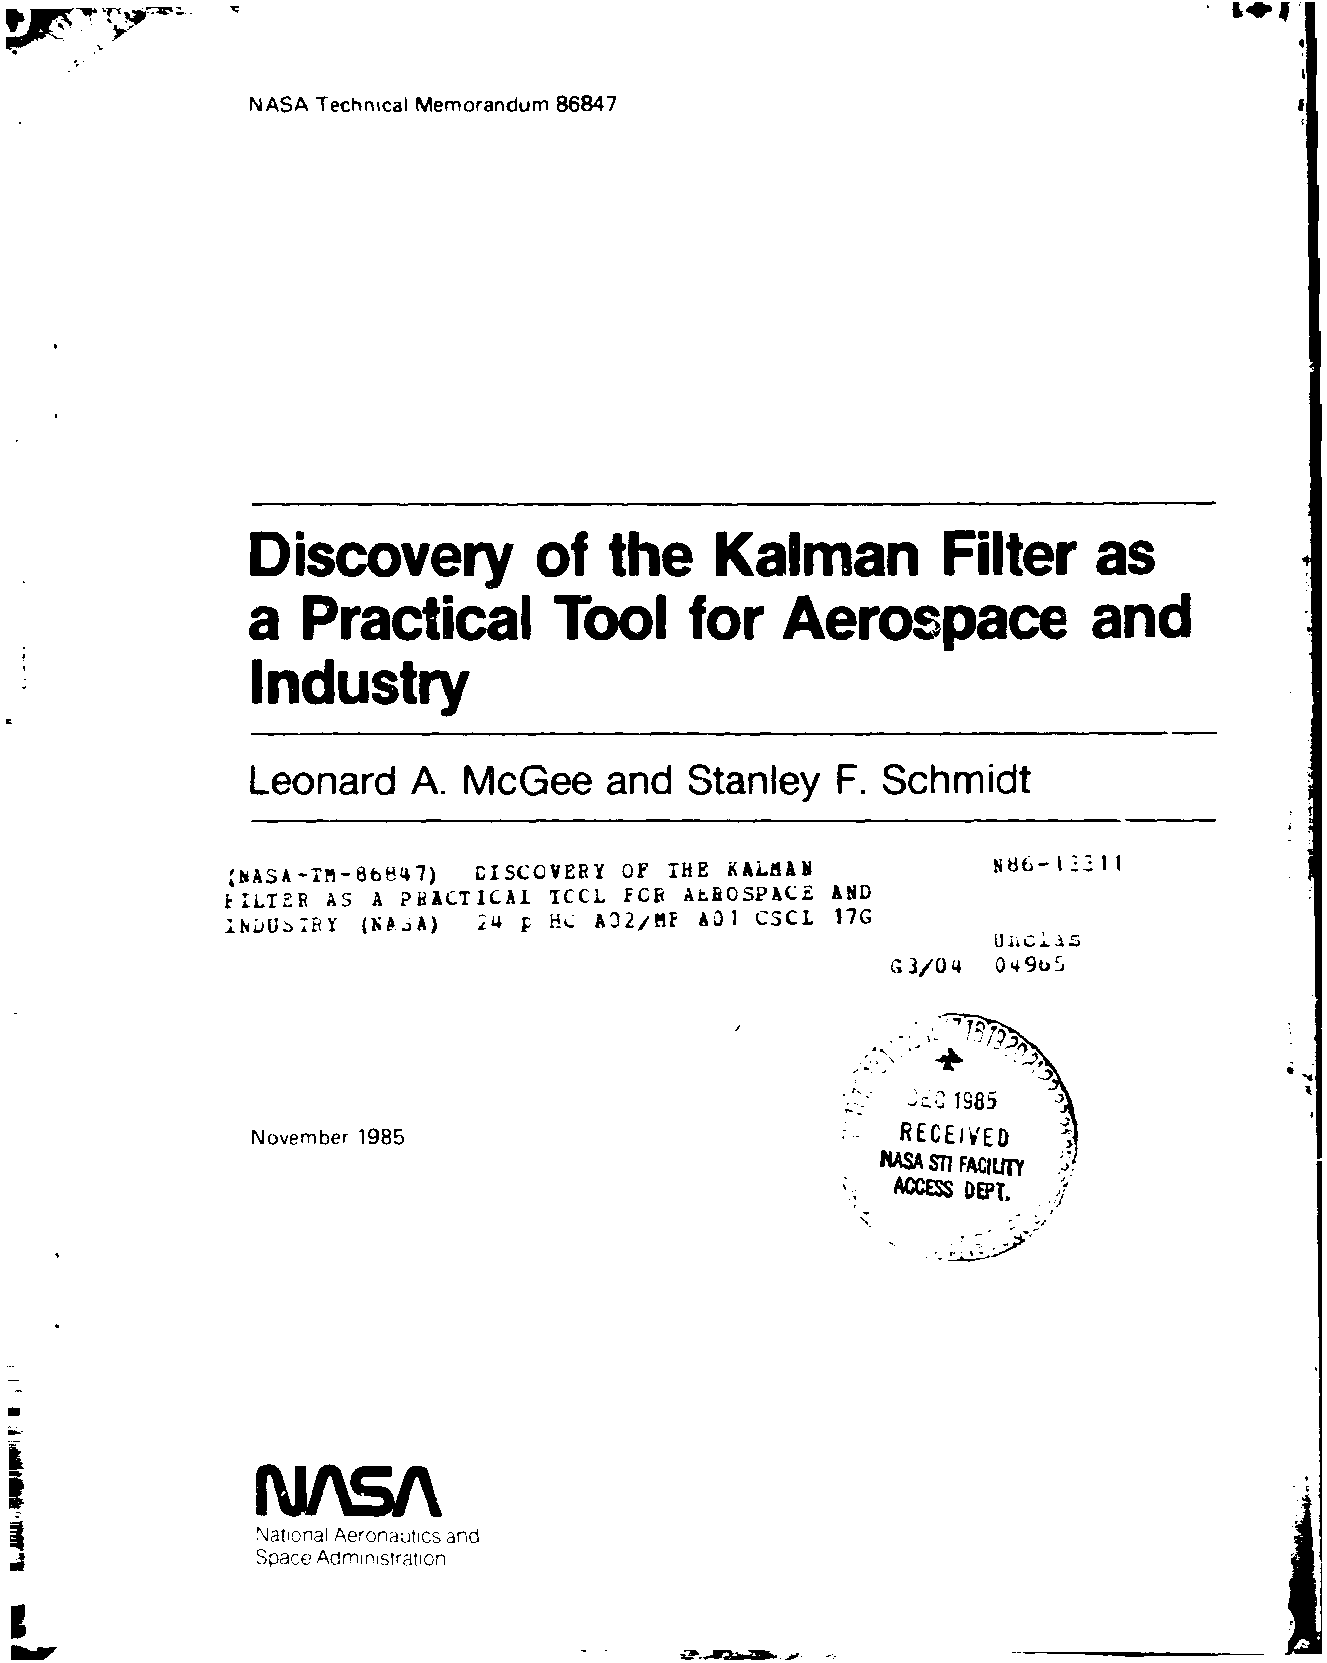
\includegraphics[width=0.80\textwidth]{Figures/Part3/Discovery of the Kalman Filter as a Practical Tool for Aerospace and Industry - NASA - Cover.pdf}
				\label{fig:Schmit_NASA}
			\end{figure}
		\end{columns}

\vspace{10pt}
    * {\tiny[Encounters and Interactions with Rudolf E. Kalman, Thomas Kailith]}
\end{frame}


\begin{frame}
   \frametitle{Kalman Filter Extensions}
   \begin{itemize}
    \item Kalman--Bucy Filter (Continuous time)
    \item \textbf{Extended Kalman Filter (EKF)}
    \item Distributed Kalman Filter
    \item \textbf{Unscented Kalman Filter}
    \item Discriminative Kalman Filter
    \item Adaptive Kalman Filter
    \item Hybrid Kalman Filter
    \item $\cdots$
   \end{itemize}
\end{frame}


%-----------------------------------------------
\subsection{Extended Kalman Filter (EKF)}
\begin{frame}{Extended Kalman Filter (EKF)---Analytic linearization}
    The main idea behind the EKF is the linearization of the dynamic model at the working point.

    \begin{figure}
        \centering
        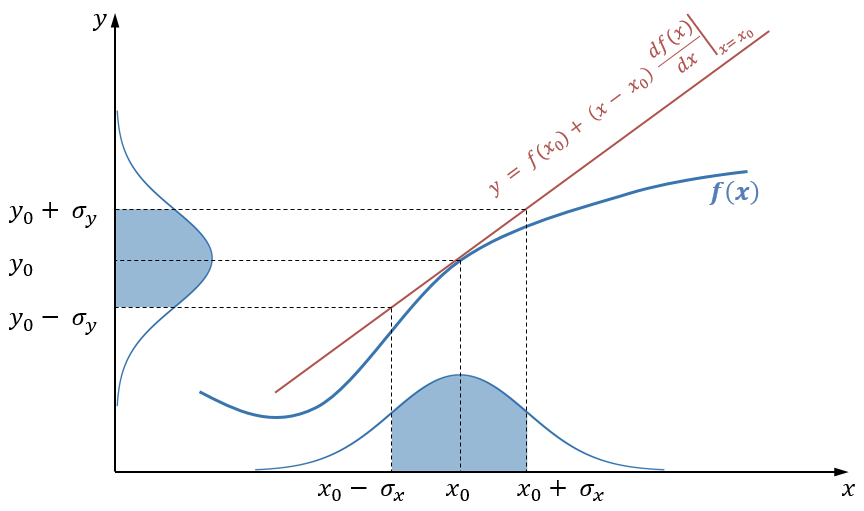
\includegraphics[width=0.65\linewidth]{Figures//Part3/1D_AnalyticLinearization.png}
        \caption{One-dimensional case for analytic linearization of the model at each point in time}
        \label{fig:enter-label}
    \end{figure}

    Using the tangent line at a point $x = x_0$, we can project the uncertainty to the y-axis and keep its’ shape Gaussian.
\end{frame}

%%%%%%%%%%%%%%%%%%%%%%%%%%%%%%%%%%%%%%%%%%%%%%
\subsubsection{Analytic linearization}
\begin{frame}{Analytic linearization}
\begin{columns}
\column{0.5\textwidth}
\begin{itemize}
    \item The slope ($m$) of the tangent line to the function $f(x)$ at the point $x_0$ equals to the derivative of the function $f(x)$ at the point $x_0$:
\[
m = \left. \frac{df(x)}{dx} \right|_{x = x_0}
\]

\item The general straight-line equation is:
\[
y = mx + b 
\]

\item We can find the line equation given the slope \( m \) and any point \( (x_0, y_0) \):
\[
y - y_0 = m(x - x_0) 
\]

\item Expand and rearrange:
\[
\begin{aligned}
y &= mx \underset{b}{\,\,\underbrace{-mx_0 + y_0}} \quad (1)
\end{aligned}
\]

\item We can find \( y_0 \) using the original function \( f(x) \):
\[
y_0 = f(x_0)
\]
\end{itemize}

\column{0.5\textwidth}
\begin{itemize}
    \item The tangent line equation, using (1), is
    \[
\begin{aligned}
y &= mx - mx_0 + y_0 \\
  &= y_0 + (x - x_0)m \\
  &= f(x_0) + (x - x_0) \left. \frac{df(x)}{dx} \right|_{x = x_0} \\
  &= f(x_0) + f(x)'(x - x_0)
\end{aligned}
\]
\end{itemize}

\end{columns}
\end{frame}

%%%%%%%%%%%%%%%%%%%%%%%%%%%%%%%%%%%%%%%%%%%%%%
\subsubsection{First-order Taylor series expansion}
\begin{frame}{First-order Taylor series expansion}
The process of analytic linearization is also called:
``The approximation of $f(x)$ by a first-order Taylor series expansion about the point $x = x_0$."

\begin{itemize}
    \item According to Taylor’s theorem, the function $f(x)$ equals an infinite sum of terms that are expressed in terms of the function derivatives at a single point $x = x_0$:
\[
f(x) \approx f(x_0) + f'(x_0)(x - x_0) + \frac{f''(x_0)}{2!}(x - x_0)^2 + \frac{f'''(x_0)}{3!}(x - x_0)^3 + \cdots + \frac{f^{(k)}(x_0)}{k!}(x - x_0)^k + \cdots
\]

\item We can approximate the function $f(x)$ by calculating the first $k$ terms of the Taylor Series. For high approximation precision, we shall select a high $k$ value. 

\item For the linear approximation, we should keep only the first two terms of the Taylor Series:
\[
f(x) \approx f(x_0) + f'(x_0)(x - x_0)
\]
\end{itemize}
\end{frame}


%%%%%%%%%%%%%%%%%%%%%%%%%%%%%%%%%%%%%%%%%%%%%%
\subsubsection{Uncertainty Projection}
\begin{frame}{Uncertainty Projection in One Dimension}

\begin{columns}
\column{0.5\textwidth}
\begin{itemize}
    \item The EKF projects the uncertainty using the linearization technique.

    \item When projecting the uncertainty, there is no need to evaluate the observation function $h(x)$ and the state transition function $f(x)$. Intead, we only need to evaluate derivatives $\frac{dh(x)}{dx}$ and $\frac{df(x)}{dx}$.

    \item After finding the tangent line equation at the point $x_0$, we can project the uncertainty using the tangent line.

    \item The line equation is:
    \vspace{-8pt}
    \[
    y = mx + b
    \]
    \[
    m = \left. \frac{df(x)}{dx} \right|_{x = x_0}
    \]
    \[
    b = -mx_0 + y_0
    \]
    \item The standard deviation (sigma) points are: $(x_0 + \sigma_x, x_0 - \sigma_x)$.
    \vspace{-8pt}
    \[
    y - \sigma_y = m(x_0 - \sigma_x) + b
    \]
    \[
    y + \sigma_y = m(x_0 + \sigma_x) + b
    \]
\end{itemize}

\column{0.5\textwidth}
\begin{itemize}
    \item The measurement uncertainty is the difference between the sigma points:
\begin{align*}
    & (y + \sigma_y)  - (y - \sigma_y) = \\
    & m(x_0 + \sigma_x) + b - (m(x_0 - \sigma_x) + b)
\end{align*}
\end{itemize}


\[
\Rightarrow \sigma_y = m\sigma_x = \left| \frac{df(x)}{dx} \right| \sigma_x
\]

The estimation variance: $p_x = \sigma_x^2$ 
\[
p_y = \left| \frac{df(x)}{dx} \right|^2 p_x
\]

\end{columns}
\end{frame}


%%%%%%%%%%%%%%%%%%%%%%%%%%%%%%%%%%%%%%%%%%%%%%
\begin{frame}{Example – linearization in a single dimension}
\begin{columns}
\column{0.5\textwidth}
\begin{itemize}
    \item Recall balloon altitude measurement example with a state-to-measurement non-linear relation.
    \item The balloon altitude is measured by the optical sensor that is located aside. The distance $d$ between the sensor and the nadir of the balloon is known. The optical sensor can measure the target angle $\theta$.
    \item The measurement equation has the following form $z_n = h(x_n)$, i.e., 
    \[
z_n = \theta = \tan^{-1} \frac{x_n}{d}
\]
\[
h(x_n) = \theta = \tan^{-1} \frac{x_n}{d}
\]

    \item To propagate the measurement uncertainty from the angle domain to the altitude domain using analytic linearization, i.e., differentiate $h(x_n)$.
    \[
\frac{dh(x)}{dx} = \frac{d}{dx} \left( \tan^{-1} \frac{x}{d} \right)
\]
\end{itemize}

\column{0.5\textwidth}
\begin{itemize}
    \item The derivative of the arctan is given by:
\begin{align*}
    & \frac{d}{dx} \tan^{-1}(x)  = \frac{1}{1 + x^2} \\
& \Rightarrow 
\frac{dh(x)}{dx} = \left[ \frac{d}{d^2 + x^2} \right]
\end{align*}
\end{itemize} 
\begin{figure}
    \centering
    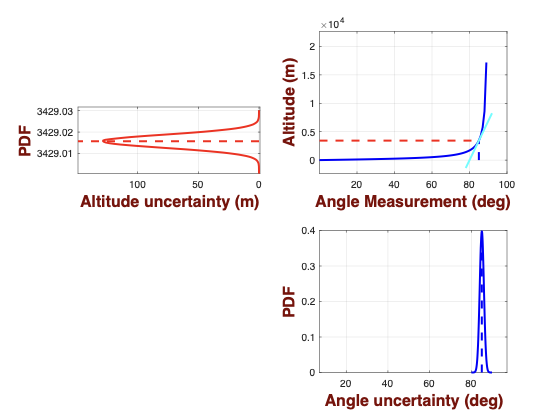
\includegraphics[width=0.95\linewidth]{Figures//Part3/Balloon_Linearization.png}
    \vspace{-10pt}
    \caption{Linearization example with tangent line to the function $x = d \cdot tan(\theta)$ at the point $\theta=85^o$.}
    \label{fig:enter-label}
\end{figure}
\end{columns}

\texttt{\tiny [Code: Non-linear KF/Balloon\_State2MeasurementUncertainty\_Linearization.m]}

\end{frame}


%%%%%%%%%%%%%%%%%%%%%%%%%%%%%%%%%%%%%%%%%%%%%%
\begin{frame}{Uncertainty projection in two dimensions}
\begin{columns}
\column{0.5\textwidth}
\begin{itemize}
    \item In two dimensions, the uncertainty is projected through a tangent plane.
\begin{figure}
    \centering
    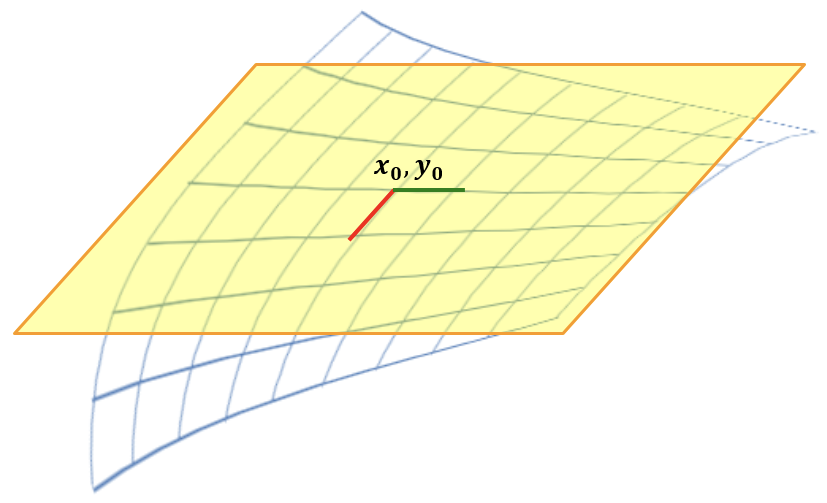
\includegraphics[width=0.95\linewidth]{Figures//Part3/TangentPlane.png}
    \caption{Tangent plane: An example of a tangent plane of the non-linear function $f(x, y)$ at a point $x0, y0$.}
    \label{fig:enter-label}
    \vspace{-10pt}
\end{figure}
\item The tangent plane is characterized by two orthogonal slopes – the x-axis slope and the y-axis slope. The partial derivatives of \( f(x, y) \) at a point \( (x_0, y_0) \) are the slopes of the tangent plane:
\[
\frac{\partial f(x, y)}{\partial x}, \quad \frac{\partial f(x, y)}{\partial y}
\]
\end{itemize}
\column{0.5\textwidth}
\begin{itemize}
    \item  In two dimensions also, we need to find two partial derivatives for projecting the uncertainty.
    \item For the pendulum example, the state vector of the pendulum is
    \[
    \mathbf{x}_n =
    \begin{bmatrix}
    \theta_n \\
    \dot{\theta}_n
    \end{bmatrix}
    \]
    \vspace{-8pt}
\begin{itemize}
    \item $\theta_n$ is the pendulum angle at time $n$
    \item $\dot{\theta}_n$ is the pendulum angular velocity at time $n$
\end{itemize}

\item We measure the pendulum position: $L \cdot \sin(\theta_n)$.

\item Since the s\textbf{tate-to-measurement relation is non-linear}, the measurement equation is a type of:
\[
\mathbf{z}_n = \mathbf{h}(\mathbf{x}_n)
\]
\[
\mathbf{h}(\mathbf{x}_n) = L \cdot \sin(\theta_n)
\]

\item The multivariate analytical linearization is:
\[
\mathbf{P}_{\text{out}} = \frac{\partial \mathbf{h}}{\partial \mathbf{x}} \mathbf{P}_{\text{in}} \left( \frac{\partial \mathbf{h}}{\partial \mathbf{x}} \right)^T
\]

\end{itemize}
\end{columns}
\end{frame}


%%%%%%%%%%%%%%%%%%%%%%%%%%%%%%%%%%%%%%%%%%%%%%
\begin{frame}{Multivariate uncertainty projection}
\begin{columns}
\column{0.5\textwidth}
\begin{itemize}
    \item We must find the partial derivatives of $h(\mathbf{x})$:
\[
\frac{\partial \mathbf{h}}{\partial \mathbf{x}} =
\begin{bmatrix}
\frac{\partial (L \sin(\theta_n))}{\partial \theta} & \frac{\partial (L \sin(\theta_n))}{\partial \dot{\theta}}
\end{bmatrix}
=
\begin{bmatrix}
L \cos(\theta_n) & 0
\end{bmatrix}
\]
\[
\mathbf{P}_{\text{out}} = \frac{\partial \mathbf{h}}{\partial \mathbf{x}} \mathbf{P}_{\text{in}} \left( \frac{\partial \mathbf{h}}{\partial \mathbf{x}} \right)^T = (L \cos(\theta_n))^2 \mathbf{P}_{\text{in}}
\]

\end{itemize}

\textbf{The dynamic model of the pendulum is also non-linear}(the second type of non-linearity). It has the form of:
\[
\hat{\mathbf{x}}_{n+1,n} = \mathbf{f}(\hat{\mathbf{x}}_{n,n})
\]
\[
\hat{\mathbf{x}}_{n+1,n} =
\begin{bmatrix}
\hat{\theta}_{n+1,n} \\
\hat{\dot{\theta}}_{n+1,n}
\end{bmatrix}
=
\begin{bmatrix}
\hat{\theta}_{n,n} + \hat{\dot{\theta}}_{n,n} \Delta t \\
\hat{\dot{\theta}}_{n,n} - \frac{g}{L} \sin(\hat{\theta}_{n,n}) \Delta t
\end{bmatrix}
\]
\[
\mathbf{f}(\hat{\mathbf{x}}_{n,n}) =
\begin{bmatrix}
f_1(\hat{\mathbf{x}}_{n,n}) \\
f_2(\hat{\mathbf{x}}_{n,n})
\end{bmatrix}
=
\begin{bmatrix}
\hat{\theta}_{n,n} + \hat{\dot{\theta}}_{n,n} \Delta t \\
\hat{\dot{\theta}}_{n,n} - \frac{g}{L} \sin(\hat{\theta}_{n,n}) \Delta t
\end{bmatrix}
\]

\begin{itemize}
    \item The dynamic model function $f(\hat{\mathbf{x}}_{n,n})$ is a matrix that contains two different sub-functions. We should find partial derivatives for each sub-function.
\end{itemize}


\column{0.5\textwidth}
\begin{align*}
 \frac{\partial \mathbf{f}(\mathbf{x})}{\partial \mathbf{x}} & =
\begin{bmatrix}
\frac{\partial f_1}{\partial \hat{\theta}} & \frac{\partial f_1}{\partial \hat{\dot{\theta}}} \\
\frac{\partial f_2}{\partial \hat{\theta}} & \frac{\partial f_2}{\partial \hat{\dot{\theta}}}
\end{bmatrix} \\ &=
\begin{bmatrix}
\frac{\partial (\hat{\theta}_{n,n} + \hat{\dot{\theta}}_{n,n} \Delta t)}{\partial \hat{\theta}} & \frac{\partial (\hat{\theta}_{n,n} + \hat{\dot{\theta}}_{n,n} \Delta t)}{\partial \hat{\dot{\theta}}} \\
\frac{\partial (\hat{\dot{\theta}}_{n,n} - \frac{g}{L} \sin(\hat{\theta}_{n,n}) \Delta t)}{\partial \hat{\theta}} & \frac{\partial (\hat{\dot{\theta}}_{n,n} - \frac{g}{L} \sin(\hat{\theta}_{n,n}) \Delta t)}{\partial \hat{\dot{\theta}}}
\end{bmatrix} \\ &=
\begin{bmatrix}
1 & \Delta t \\
-\frac{g}{L} \cos(\hat{\theta}_{n,n}) \Delta t & 1
\end{bmatrix}
\end{align*}

The multivariate analytical linearization is given by:
\[
\mathbf{P}_{\text{out}} = \frac{\partial \mathbf{f}}{\partial \mathbf{x}} \mathbf{P}_{\text{in}} \left( \frac{\partial \mathbf{f}}{\partial \mathbf{x}} \right)^T
\]
\end{columns}
\end{frame}


%%%%%%%%%%%%%%%%%%%%%%%%%%%%%%%%%%%%%%%%%%%%%%
\begin{frame}{Multivariate uncertainty projection}

\begin{itemize}
    \item We can generalize the two-dimensional case by extending it to an $N$ - dimensional
case.
\item For multi-dimensional problems, we propagate the multivariate Gaussian random
variable (represented by covariance matrix) using a linear approximation of the
multi-dimensional function.
\item For the non-linear system dynamics, the multivariate analytical linearization is given
by:
\[
\mathbf{P}_{\text{out}} = \dfrac{\partial \mathbf{f}}{\partial \mathbf{x}} \mathbf{P}_{\text{in}} \left( \dfrac{\partial \mathbf{f}}{\partial \mathbf{x}} \right)^T
\]
where $\dfrac{\partial \mathbf{f}}{\partial \mathbf{x}}$ is state transition matrix Jacobian.

\item Similarly, for the state-to-measurement non-linear relation, the multivariate analytical
linearization is given by:
\[
\mathbf{P}_{\text{out}} = \dfrac{\partial \mathbf{h}}{\partial \mathbf{x}} \mathbf{P}_{\text{in}} \left( \dfrac{\partial \mathbf{h}}{\partial \mathbf{x}} \right)^T
\]
where $\dfrac{\partial \mathbf{h}}{\partial \mathbf{x}}$ an observation matrix Jacobian.
 \end{itemize}

For additional material on error propagation refer to \cite{fx1998introduction}.
\end{frame}


%%%%%%%%%%%%%%%%%%%%%%%%%%%%%%%%%%%%%%%%%%%%%%
\begin{frame}{Jacobian derivation example}
\vspace{-5pt}
\begin{columns}
\column{0.5\textwidth}
Let's refer back to “Vehicle location estimation example” Slide~\ref{subsec:Ex9}, where we estimated the vehicle location in the XY plane using onboard location sensor, reported \(x\) and \(y\) coordinates.
\vspace{5pt}

Now, we want to track the vehicle using radar, located at the plane origin, measuring the vehicle range (\(r\)) and bearing angle (\(\phi\)). The radar measurement error distribution is Gaussian.
\vspace{-7pt}
\begin{figure}
    \centering
    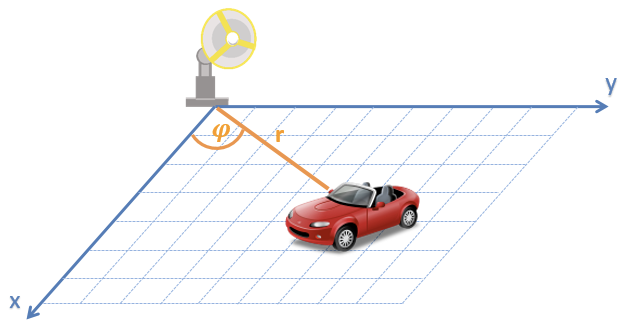
\includegraphics[width=0.4\linewidth]{Figures//Part3/VehicleLocation_Radar.png}
    \vspace{-8pt}
    \caption{Vehicle location estimation using radar.}
    \label{fig:enter-label}
    \vspace{-14pt}
\end{figure}

\begin{itemize}
    \item The measurement vector \(\mathbf{z}_n\) and the state vector \(\mathbf{x}_n\) is:
\[
\mathbf{z}_n =
\begin{bmatrix}
r_n \\
\phi_n
\end{bmatrix}, \quad \mathbf{x}_n =
\begin{bmatrix}
x_n \\
y_n
\end{bmatrix}
\]
% \item The state vector \(x_n\) is:
% \[
% x_n =
% \begin{bmatrix}
% x_n \\
% y_n
% \end{bmatrix}
% \]
\item Let us find the relation between the measurement vector and the state vector. The vehicle range (\(r\)) can be expressed by \(x\) and \(y\) as:
    \[
    r = \sqrt{x^2 + y^2}
    \]
\end{itemize}

\column{0.5\textwidth}
\begin{itemize}
    
    \item The vehicle bearing angle (\(\phi\)) can be expressed by \(x\) and \(y\) as:
\[
\phi = \tan^{-1} \left(\frac{y}{x}\right)
\]

\item Since the state-to-measurement relation is non-linear, the measurement equation is a type of \(\mathbf{z}_n = \mathbf{h}(x_n)\):
\[
\begin{bmatrix}
r \\
\phi
\end{bmatrix}
=
\begin{bmatrix}
\sqrt{x^2 + y^2} \\
\tan^{-1} \left(\frac{y}{x}\right)
\end{bmatrix}
\]
\end{itemize}
Jacobian derivation:
\[
\frac{\partial h}{\partial x} =\!\!
\begin{bmatrix}
\frac{\partial h_1}{\partial x_1} & \!\!\!\!\cdots \!\!\!\!& \frac{\partial h_1}{\partial x_n} \\
\vdots & \ddots & \vdots \\
\frac{\partial h_m}{\partial x_1} & \!\!\!\! \cdots \!\!\!\!& \frac{\partial h_m}{\partial x_n}
\end{bmatrix}
\!\!=\!\!
\begin{bmatrix}
\frac{\partial \sqrt{x^2 + y^2}}{\partial x} \!\!&\!\! \frac{\partial \sqrt{x^2 + y^2}}{\partial y} \\
\frac{\partial \tan^{-1} \left(\frac{y}{x}\right)}{\partial x} \!\!&\!\! \frac{\partial \tan^{-1} \left(\frac{y}{x}\right)}{\partial y}
\end{bmatrix}
\]

\[
\frac{\partial \mathbf{h}(\mathbf{x})}{\partial \mathbf{x}} =
\begin{bmatrix}
\frac{x}{\sqrt{x^2 + y^2}} & \frac{y}{\sqrt{x^2 + y^2}} \\
-\frac{y}{x^2 + y^2} & \frac{x}{x^2 + y^2}
\end{bmatrix}
\]

\end{columns}
\end{frame}


%%%%%%%%%%%%%%%%%%%%%%%%%%%%%%%%%%%%%%%%%%%%%%
\subsubsection{EKF Equations}
\begin{frame}{EKF Equations---The EKF observation matrix - $\mathbf{H}$}

EK requires modifications related to the observation matrix $\mathbf{H}$ and the state transition matrix $\mathbf{F}$.

If the state-to-measurement relation (the first type of non-linearity) of the system is
non-linear, the observation matrix is of the type
\[
\mathbf{H} = \mathbf{h}(\mathbf{x}_n)
\]
The State Update Equation looks like the following:
\[
\hat{\mathbf{x}}_{n,n} = \hat{\mathbf{x}}_{n,n-1} + \mathbf{K}_n (\mathbf{z}_n - \textcolor{blue}{\mathbf{h}(\hat{\mathbf{x}}_{n,n-1})})
\]

For the uncertainty propagation, the observation matrix \(\mathbf{H}\) should be linearized to keep the uncertainty PDF Gaussian, Therefore, the \textbf{Covariance Update Equation} looks like the following:
\[
\mathbf{P}_{n,n} = \left( \mathbf{I} - \mathbf{K}_n \textcolor{blue}{\frac{\partial \mathbf{h}}{\partial \mathbf{x}}} \right) \mathbf{P}_{n,n-1} \left( \mathbf{I} - \mathbf{K}_n \textcolor{blue}{\frac{\partial \mathbf{h}}{\partial \mathbf{x}}} \right)^T + \mathbf{K}_n \mathbf{R}_n \mathbf{K}_n^T
\]

The Kalman Gain Equation looks like the following:
\[
\mathbf{K}_n = \mathbf{P}_{n,n-1} \textcolor{blue}{\left( \frac{\partial \mathbf{h}}{\partial \mathbf{x}} \right)^T} \left( \textcolor{blue}{\frac{\partial \mathbf{h}}{\partial \mathbf{x}}} \mathbf{P}_{n,n-1} {\left( \frac{\partial \mathbf{h}}{\partial \mathbf{x}} \right)^T} + \mathbf{R}_n \right)^{-1}
\]
\end{frame}


%%%%%%%%%%%%%%%%%%%%%%%%%%%%%%%%%%%%%%%%%%%%%%
\begin{frame}{EKF Equations---The EKF state transition matrix $\mathbf{F}$}

If the dynamic model (the second type of non-linearity) of the system is non-linear,
the observation matrix is of the type:
\[
\mathbf{F} = \mathbf{f}(\mathbf{x}_n)
\]

For the uncertainty propagation, the state transition matrix \(\mathbf{F}\) should be linearized to keep the uncertainty PDF Gaussian. The State Extrapolation Equation looks like the following:
\[
\hat{\mathbf{x}}_{n+1,n} = \mathbf{f}(\hat{\mathbf{x}}_{n,n}) + \mathbf{G} \mathbf{u}_n
\]

The Covariance Extrapolation Equation looks like the following:
\[
\mathbf{P}_{n+1,n} = \textcolor{red}{\frac{\partial \mathbf{f}}{\partial \mathbf{x}}} \mathbf{P}_{n,n} \textcolor{red}{\left( \frac{\partial \mathbf{f}}{\partial \mathbf{x}} \right)^T} + \mathbf{Q}
\]
\end{frame}


%%%%%%%%%%%%%%%%%%%%%%%%%%%%%%%%%%%%%%%%%%%%%%
\begin{frame}{Summary of EKF Equations}
\begin{figure}
    \centering
    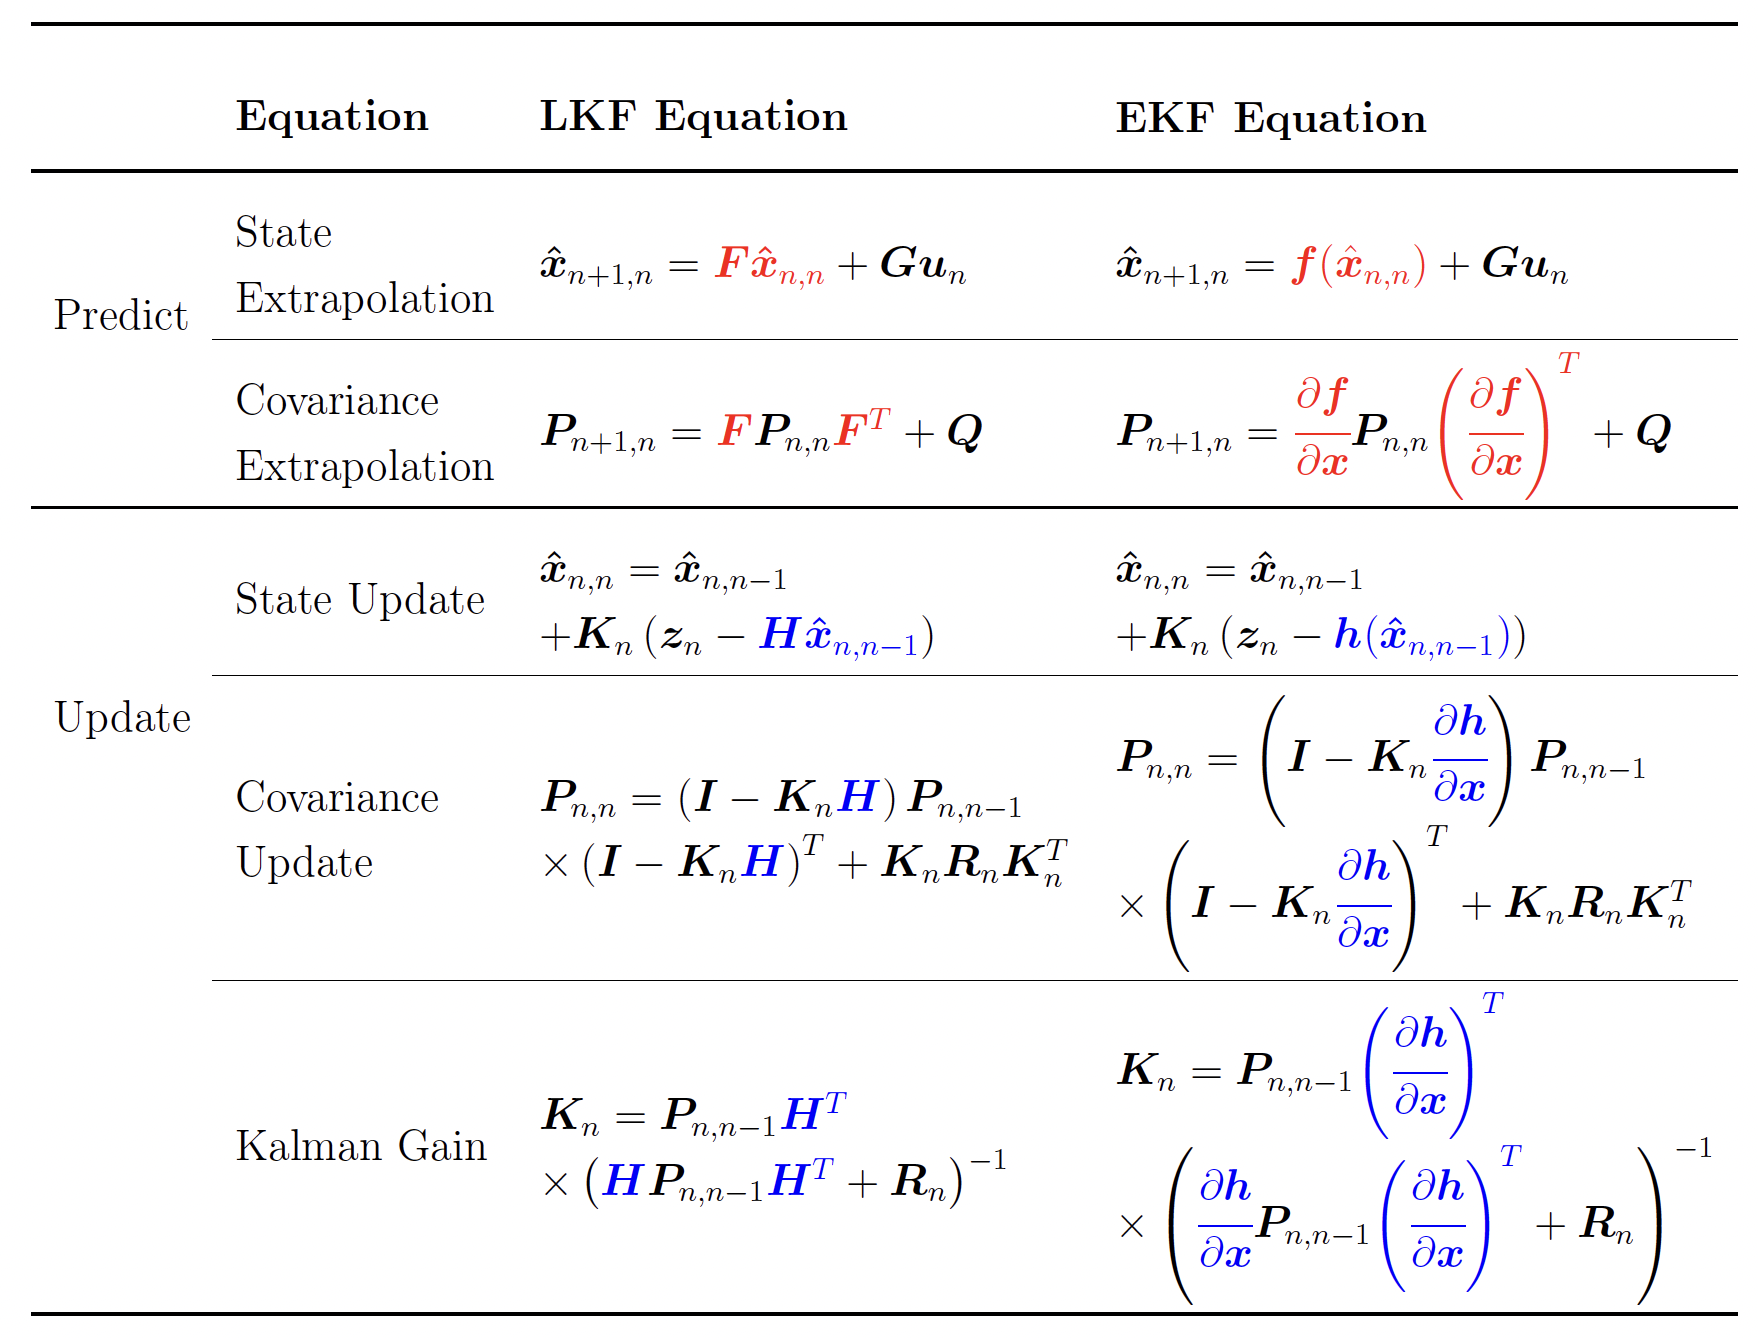
\includegraphics[width=0.85\linewidth]{Figures//Part3/EKF_Eq_Summary.png}
    \caption{Summary of EKF Equations}
    \label{fig:Summary_EKF_Equations}
\end{figure}
\end{frame}

%%%%%%%%%%%%%%%%%%%%%%%%%%%%%%%%%%%%%%%%%%%%%%
\subsubsection{Example 11 – vehicle location estimation using radar}
\begin{frame}{Example 11 – vehicle location estimation using radar}
\label{Example11}
\vspace{-7pt}
\begin{columns}
\column{0.4\textwidth}
\begin{itemize}
    \item We want to track the vehicle using radar, which is located at the plane origin, measuring the vehicle range ($r$) and the bearing angle ($\varphi$).
    \item The radar measurement error distribution is Gaussian. 
\end{itemize}
Let's look at KF equations.

\textbf{The state extrapolation equation}
\begin{itemize}
    \item The state extrapolation equation:
\[
\hat{\mathbf{x}}_{n+1,n} = \mathbf{F} \hat{\mathbf{x}}_{n,n}
\]

The system state \(\mathbf{x}_n\) is defined by:
\[
\mathbf{x}_n =
\begin{bmatrix}
x_n \\
\dot{x}_n \\
\ddot{x}_n \\
y_n \\
\dot{y}_n \\
\ddot{y}_n
\end{bmatrix}
\]
\end{itemize}


\column{0.6\textwidth}
\begin{itemize}
    \item Assuming constant acceleration dynamics, the extrapolated vehicle state for time \(n + 1\) can be described as:
    \vspace{-5pt}
\[\!\!\!\!
\begin{bmatrix}
\hat{x}_{n+1,n} \\
\hat{\dot{x}}_{n+1,n} \\
\hat{\ddot{x}}_{n+1,n} \\
\hat{y}_{n+1,n} \\
\hat{\dot{y}}_{n+1,n} \\
\hat{\ddot{y}}_{n+1,n}
\end{bmatrix}
\!\!=\!\!
\begin{bmatrix}
1 & \Delta t & 0.5\Delta t^2 & 0 & 0 & 0 \\
0 & 1 & \Delta t & 0 & 0 & 0 \\
0 & 0 & 1 & 0 & 0 & 0 \\
0 & 0 & 0 & 1 & \Delta t & 0.5\Delta t^2 \\
0 & 0 & 0 & 0 & 1 & \Delta t \\
0 & 0 & 0 & 0 & 0 & 1
\end{bmatrix}\!\!
\begin{bmatrix}
\hat{x}_{n,n} \\
\hat{\dot{x}}_{n,n} \\
\hat{\ddot{x}}_{n,n} \\
\hat{y}_{n,n} \\
\hat{\dot{y}}_{n,n} \\
\hat{\ddot{y}}_{n,n}
\end{bmatrix}
\]
\vspace{-7pt}
\item The dynamic model of the system (the second type of non-linearity) in this example is linear! There is no need to calculate the Jacobian \(\dfrac{\partial \mathbf{f}}{\partial \mathbf{x}}\).

\textbf{The covariance extrapolation equation} is similar to example 9~\ref{subsec:Ex9}:
\vspace{-7pt}
\[
\mathbf{P}_{n+1,n} = \mathbf{F} \mathbf{P}_{n,n} \mathbf{F}^T + \mathbf{Q}
\]
\vspace{-5pt}
The estimate covariance is:
\vspace{-5pt}
\[
\mathbf{P} =
\begin{bmatrix}
p_{x} & p_{x\dot{x}} & p_{x\ddot{x}} & 0 & 0 & 0 \\
p_{\dot{x}x} & p_{\dot{x}} & p_{\dot{x}\ddot{x}} & 0 & 0 & 0 \\
p_{\ddot{x}x} & p_{\ddot{x}\dot{x}} & p_{\ddot{x}} & 0 & 0 & 0 \\
0 & 0 & 0 & p_{y} & p_{y\dot{y}} & p_{y\ddot{y}} \\
0 & 0 & 0 & p_{\dot{y}y} & p_{\dot{y}} & p_{\dot{y}\ddot{y}} \\
0 & 0 & 0 & p_{\ddot{y}y} & p_{\ddot{y}\dot{y}} & p_{\ddot{y}}
\end{bmatrix}
\]
\end{itemize}
\end{columns}
\end{frame}

%%%%%%%%%%%%%%%%%%%%%%%%%%%%%%%%%%%%%%%%%%%%%%
\begin{frame}{Example 11 – vehicle location estimation using radar}
\begin{columns}
\column{0.5\textwidth}
The process noise matrix is also similar to example 9:
\begin{align*}
\mathbf{Q} & =
\begin{bmatrix}
\sigma^2_{x} & \sigma^2_{x\dot{x}} & \sigma^2_{x\ddot{x}} & 0 & 0 & 0 \\
\sigma^2_{\dot{x}x} & \sigma^2_{\dot{x}} & \sigma^2_{\dot{x}\ddot{x}} & 0 & 0 & 0 \\
\sigma^2_{\ddot{x}x} & \sigma^2_{\ddot{x}\dot{x}} & \sigma^2_{\ddot{x}} & 0 & 0 & 0 \\
0 & 0 & 0 & \sigma^2_{y} & \sigma^2_{y\dot{y}} & \sigma^2_{y\ddot{y}} \\
0 & 0 & 0 & \sigma^2_{\dot{y}y} & \sigma^2_{\dot{y}} & \sigma^2_{\dot{y}\ddot{y}} \\
0 & 0 & 0 & \sigma^2_{\ddot{y}y} & \sigma^2_{\ddot{y}\dot{y}} & \sigma^2_{\ddot{y}}
\end{bmatrix}\\
& =
\begin{bmatrix}
\frac{\Delta t^4}{4} & \frac{\Delta t^3}{2} & \frac{\Delta t^2}{2} & 0 & 0 & 0 \\
\frac{\Delta t^3}{2} & \Delta t^2 & \Delta t & 0 & 0 & 0 \\
\frac{\Delta t^2}{2} & \Delta t & 1 & 0 & 0 & 0 \\
0 & 0 & 0 & \frac{\Delta t^4}{4} & \frac{\Delta t^3}{2} & \frac{\Delta t^2}{2} \\
0 & 0 & 0 & \frac{\Delta t^3}{2} & \Delta t^2 & \Delta t \\
0 & 0 & 0 & \frac{\Delta t^2}{2} & \Delta t & 1
\end{bmatrix}
\end{align*}


The \textbf{measurement equation} is different from example 9. The measurement vector \( \mathbf{z}_n \) is:
\[
\mathbf{z}_n =
\begin{bmatrix}
r_n \\
\phi_n
\end{bmatrix}
\]
\column{0.5\textwidth}
The system state vector \( \mathbf{x}_n \) is defined by:
\[
\mathbf{x}_n =
\begin{bmatrix}
x_n \\
\dot{x}_n \\
\ddot{x}_n \\
y_n \\
\dot{y}_n \\
\ddot{y}_n
\end{bmatrix}
\]

Let us find the relation between the measurement vector and the state vector. 
\[
r = \sqrt{x^2 + y^2}
\]
\[
\phi = \tan^{-1} \left( \frac{y}{x} \right)
\]

Since the state-to-measurement relation (the first type of non-linearity) is non-linear, the measurement equation is a type of \( \mathbf{z}_n = \mathbf{h}(\mathbf{x}_n) \):
\[
\begin{bmatrix}
r \\
\phi
\end{bmatrix}
=
\begin{bmatrix}
\sqrt{x^2 + y^2} \\
\tan^{-1} \left( \frac{y}{x} \right)
\end{bmatrix}
\]


\end{columns}
\end{frame}


%%%%%%%%%%%%%%%%%%%%%%%%%%%%%%%%%%%%%%%%%%%%%%
\begin{frame}{Example 11 – vehicle location estimation using radar}
Jacobian derivation:
\begin{align*}
\frac{\partial \mathbf{h}}{\partial \mathbf{x}} & =
\begin{bmatrix}
\frac{\partial h_1}{\partial x_1} & \cdots & \frac{\partial h_1}{\partial x_n} \\
\vdots & \ddots & \vdots \\
\frac{\partial h_m}{\partial x_1} & \cdots & \frac{\partial h_m}{\partial x_n}
\end{bmatrix}\\
& =
\begin{bmatrix}
\frac{\partial \sqrt{x^2 + y^2}}{\partial x} & \frac{\partial \sqrt{x^2 + y^2}}{\partial \dot{x}} & \frac{\partial \sqrt{x^2 + y^2}}{\partial \ddot{x}} & \frac{\partial \sqrt{x^2 + y^2}}{\partial y} & \frac{\partial \sqrt{x^2 + y^2}}{\partial \dot{y}} & \frac{\partial \sqrt{x^2 + y^2}}{\partial \ddot{y}} \\
\frac{\partial \tan^{-1} \left( \frac{y}{x} \right)}{\partial x} & \frac{\partial \tan^{-1} \left( \frac{y}{x} \right)}{\partial \dot{x}} & \frac{\partial \tan^{-1} \left( \frac{y}{x} \right)}{\partial \ddot{x}} & \frac{\partial \tan^{-1} \left( \frac{y}{x} \right)}{\partial y} & \frac{\partial \tan^{-1} \left( \frac{y}{x} \right)}{\partial \dot{y}} & \frac{\partial \tan^{-1} \left( \frac{y}{x} \right)}{\partial \ddot{y}}
\end{bmatrix}\\
& = 
\frac{\partial \mathbf{h}}{\partial \mathbf{x}} =
\begin{bmatrix}
\frac{x}{\sqrt{x^2 + y^2}} & 0 & 0 & \frac{y}{\sqrt{x^2 + y^2}} & 0 & 0 \\
-\frac{y}{x^2 + y^2} & 0 & 0 & \frac{x}{x^2 + y^2} & 0 & 0
\end{bmatrix}
\end{align*}
The \textbf{measurement uncertainty} is represented by the measurement covariance matrix:
\[
\mathbf{R}_n =
\begin{bmatrix}
\sigma^2_{r_m} & 0 \\
0 & \sigma^2_{\phi_m}
\end{bmatrix}
\]
The \textbf{Kalman Gain}, \textbf{The state update equation}, and \textbf{The covariance update equation} relations are the same as expressed before.
\end{frame}


%%%%%%%%%%%%%%%%%%%%%%%%%%%%%%%%%%%%%%%%%%%%%%
\begin{frame}{Example 11 – vehicle location estimation using radar: Numerical example}
\vspace{-10pt}
\begin{columns}
\column{0.5\textwidth}
\begin{itemize}
    \item The measurements period: \(\Delta t = 1\text{s}\)
    \item The random acceleration standard deviation: \(\sigma_a = 0.2\text{m/s}^2\)
    \item The range measurement error standard deviation: \(\sigma_{r_m} = 5\text{m}\)
    \item The bearing angle measurement error standard deviation: \(\sigma_{\phi_m} = 0.0087\text{rad}\)
\end{itemize}
\vspace{-15pt}
\begin{figure}
    \centering
    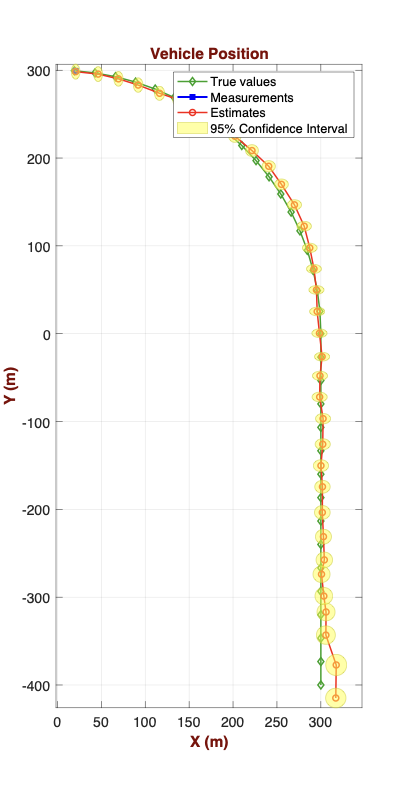
\includegraphics[width=0.45\linewidth]{Figures//Part3/ex11_VehiclePosition.png}
    \vspace{-15pt}
    \caption{True, measured, and estimated vehicle position
compared to the 95\% confidence ellipses.}
    \label{fig:ex11_Position}
\end{figure}

\column{0.5\textwidth}
\begin{figure}
    \centering
    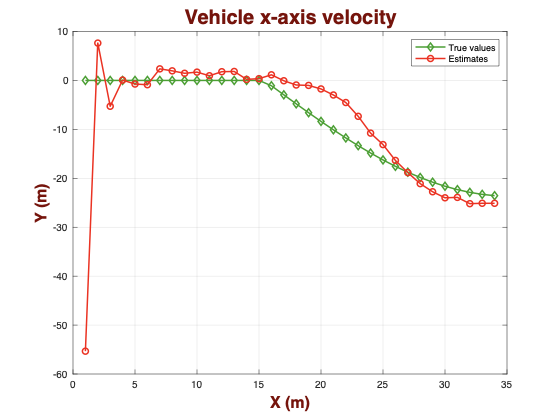
\includegraphics[width=0.9\linewidth]{Figures//Part3/ex11_x_Velocity.png}
\end{figure}
\vspace{-14pt}
\begin{figure}
    \centering
    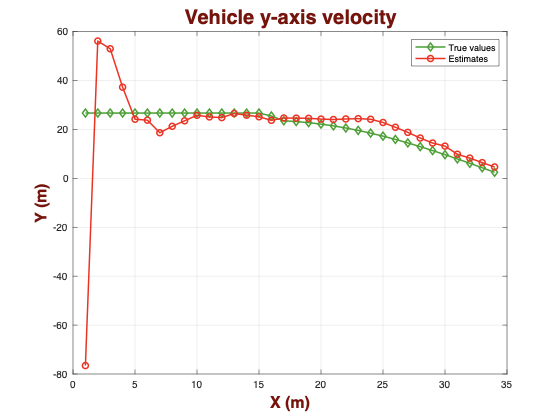
\includegraphics[width=0.9\linewidth]{Figures//Part3/ex11_y_Velocity.png}
\end{figure}
\end{columns}
\end{frame}

%%%%%%%%%%%%%%%%%%%%%%%%%%%%%%%%%%%%%%%%%%%%%%
\begin{frame}{Example 11 – vehicle location estimation using radar: Numerical example}
\vspace{-13pt}
\begin{columns}
\column{0.4\textwidth}
\begin{figure}
    \centering
    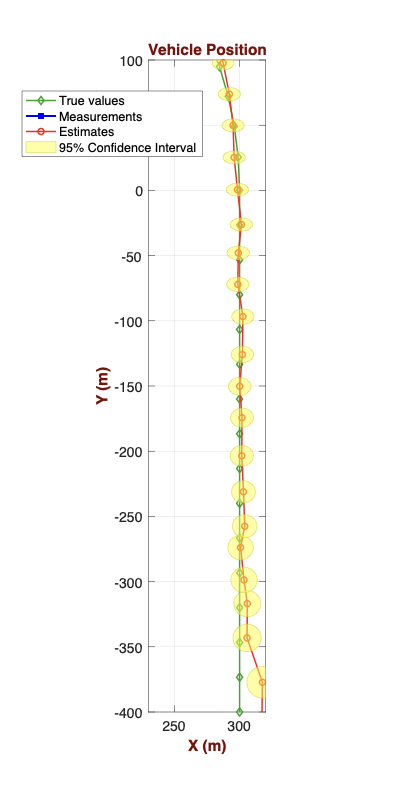
\includegraphics[width=0.9\linewidth]{Figures//Part3/ex11_Position_Straight_Zoomed.png}
\end{figure}
\column{0.6\textwidth}
\begin{figure}
    \centering
    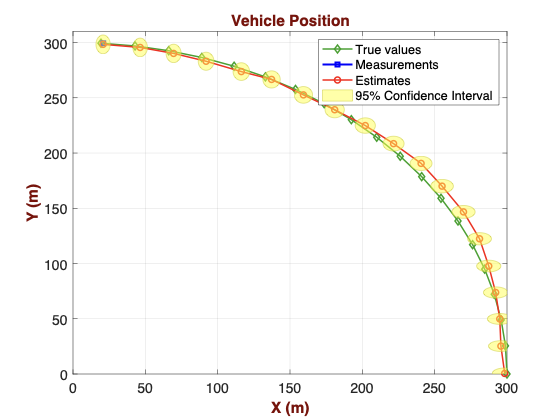
\includegraphics[width=1\linewidth]{Figures//Part3/ex11_Position_Zoom_Cureved.png}
\end{figure}

\texttt{\tiny [Code: Non-linear KF/Ex11\_EKF\_State2MeasurementUncertainty.m]}
\end{columns}
\end{frame}

%%%%%%%%%%%%%%%%%%%%%%%%%%%%%%%%%%%%%%%%%%%%%%
\subsubsection{Example 12 - estimating the pendulum angle}
\begin{frame}{Example 12 - estimating the pendulum angle}
\label{ex12}
\begin{columns}
\column{0.5\textwidth}
\begin{itemize}
    \item In this example, we want to estimate the pendulum angle $\theta$ from the measured pendulum position. 

    \item The dynamic model of the
the pendulum was derived earlier (slide XYZ). 

    \item Assume an ideal gravity
pendulum that consists of a body with mass $m$ hung by a string with length $L$ from
fixed support - the pendulum swings back and forth at a constant amplitude.

    \item We
want to estimate the angle $\theta$ from the vertical to the pendulum. The angle units are
radians.

    \item We measure the pendulum position $z = Lsin(\theta_n)$.
\end{itemize}

\column{0.5\textwidth}
\begin{figure}
    \centering
    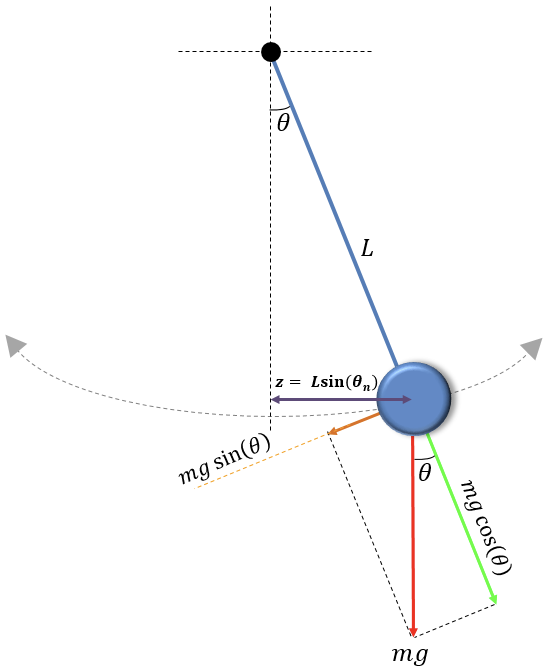
\includegraphics[width=1\linewidth]{Figures//Part3/ex12_Pendulum.png}
    \caption{Pendulum position measurement.}
\end{figure}
\end{columns}
\end{frame}


%%%%%%%%%%%%%%%%%%%%%%%%%%%%%%%%%%%%%%%%%%%%%%
\begin{frame}{Example 12 - estimating the pendulum angle: Kalman Filter Equations}
\begin{columns}
\column{0.5\textwidth}
\textbf{The State Extrapolation Equation:}
The state vector of the pendulum is:
\[
\mathbf{x}_n =
\begin{bmatrix}
\theta_n \\
\dot{\theta}_n
\end{bmatrix}
\]
where $\theta_n$ is the pendulum's angle  $\dot{\theta}_n$ the angular velocity at time $n$

The dynamic model of the pendulum is non-linear:
\[
\hat{\mathbf{x}}_{n+1,n} = \mathbf{f}(\hat{\mathbf{x}}_{n,n})
\]
\[
\hat{\mathbf{x}}_{n+1,n} =
\begin{bmatrix}
\hat{\theta}_{n+1,n} \\
\hat{\dot{\theta}}_{n+1,n}
\end{bmatrix}
=
\begin{bmatrix}
\hat{\theta}_{n,n} + \hat{\dot{\theta}}_{n,n} \Delta t \\
\hat{\dot{\theta}}_{n,n} - \frac{g}{L} \sin(\hat{\theta}_{n,n}) \Delta t
\end{bmatrix}
\]
\[
\mathbf{f}(\hat{\mathbf{x}}_{n,n}) =
\begin{bmatrix}
\hat{\theta}_{n,n} + \hat{\dot{\theta}}_{n,n} \Delta t \\
\hat{\dot{\theta}}_{n,n} - \frac{g}{L} \sin(\hat{\theta}_{n,n}) \Delta t
\end{bmatrix}
\]

\textbf{Jacobian Derivation:} The Jacobian for the pendulum dynamic model:
\[
\frac{\partial \mathbf{f}(\mathbf{x})}{\partial \mathbf{x}} =
\begin{bmatrix}
\frac{\partial f_1}{\partial \hat{\theta}} & \frac{\partial f_1}{\partial \hat{\dot{\theta}}} \\
\frac{\partial f_2}{\partial \hat{\theta}} & \frac{\partial f_2}{\partial \hat{\dot{\theta}}}
\end{bmatrix}
=
\begin{bmatrix}
1 & \Delta t \\
-\frac{g}{L} \cos(\hat{\theta}_{n,n}) \Delta t & 1
\end{bmatrix}
\]

\textbf{The Covariance Extrapolation Equation:}
is given by:
\[
\mathbf{P}_{n+1,n} = \frac{\partial \mathbf{f}(\hat{\mathbf{x}}_{n,n})}{\partial \mathbf{x}} \mathbf{P}_{n,n} \left( \frac{\partial \mathbf{f}(\hat{\mathbf{x}}_{n,n})}{\partial \mathbf{x}} \right)^T + \mathbf{Q}
\]
\column{0.5\textwidth}
\vspace*{-55pt}

The estimate covariance is:
\[
\mathbf{P} =
\begin{bmatrix}
p_{x} & p_{x\dot{x}} \\
p_{\dot{x}x} & p_{\dot{x}}
\end{bmatrix}
\]
\textbf{The Process Noise Matrix}
\[
\mathbf{Q} =
\begin{bmatrix}
\sigma^2_{x} & \sigma^2_{x\dot{x}} \\
\sigma^2_{\dot{x}x} & \sigma^2_{\dot{x}}
\end{bmatrix}
=
\begin{bmatrix}
\frac{\Delta t^4}{4} & \frac{\Delta t^3}{2} \\
\frac{\Delta t^3}{2} & \Delta t^2
\end{bmatrix}
\sigma^2_{a}
\]
\textbf{The Measurement Equation}
We measure the pendulum position: $L \sin(\theta_n)$, i.e., the state-to-measurement relation is non-linear:
\[
\mathbf{z}_n = \mathbf{h}(\mathbf{x}_n), \quad
\mathbf{h}(\mathbf{x}_n) = L \sin(\theta_n)
\]
\textbf{Jacobian Derivation} of position measurement:
\[
\frac{\partial \mathbf{h}}{\partial \mathbf{x}} =
\begin{bmatrix}
\frac{\partial (L \sin(\theta_n))}{\partial \theta}\!\! & \!\!\frac{\partial (L \sin(\theta_n))}{\partial \dot{\theta}}
\end{bmatrix}
=
\begin{bmatrix}
L \cos(\theta_n) & 0
\end{bmatrix}
\]
\textbf{The Measurement Uncertainty} is:
\[
\mathbf{R}_n =
\begin{bmatrix}
\sigma^2_{x_m}
\end{bmatrix}
\]
\end{columns}
\end{frame}

%%%%%%%%%%%%%%%%%%%%%%%%%%%%%%%%%%%%%%%%%%%%%%
\begin{frame}{Example 12 - Estimating the pendulum angle: Pendulum Motion Simulation}
\textbf{Example Parameters}
\begin{itemize}
    \item The Pendulum string length: \( L = 0.5\,\text{m} \)
    \item Gravitational acceleration constant: \( g = 9.8\,\text{m/s}^2 \)
    \item Measurement Uncertainty (standard deviation): \( \sigma_{x_m} = 0.01\,\text{m} \)
    \item Process Noise Uncertainty (angular acceleration standard deviation): \( \sigma_a = 1\,\text{rad/s}^2 \)
\end{itemize}
\textbf{Let's first do the maths for pendulum motion simulation for establish ground truth. }  
\begin{columns}
\column{0.5\textwidth}
\begin{itemize}
    \item The differential equation that describes the pendulum movement:
    $$L\frac{d^2\theta}{dt^2} = -g\sin{\theta}, \quad \text{or}~~\ddot{\theta} + \frac{g}{L} \sin\theta = 0$$
    \item \textbf{Approximation:} if $\theta$ is small, then $\sin\theta \approx \theta$, 
\[
\ddot{\theta} + \frac{g}{L} \theta = 0 \tag{E1}
\] 

\item Using "the method of inspired guessing"-- the sine and cosine functions are periodic--we can have a solution for the angle $\theta$ as a function of time $t$:
\[
\theta(t) = A \cos(\omega t) + B \sin(\omega t) \tag{E2}
\]
\end{itemize}
\column{0.5\textwidth}
\begin{itemize}
\item At $t = 0$, from E2:
\[
\theta(t = 0) = A
\]
So, $A$ is an initial angle, denoted by $\theta_0$.

\item Re-write E2:
\[
\theta(t) = \theta_0 \cos(\omega t) + B \sin(\omega t)
\]
\item The derivative of $\theta(t)$ is the angular velocity ($\omega$) of the pendulum:
\[
\omega(t) = \frac{d\theta}{dt} = \dot{\theta} = -\omega \theta_0 \sin(\omega t) + \omega B \cos(\omega t)
\]
\item To find $B$, evaluate $\omega(t)$ at $t = 0$:
\vspace{-5pt}
\[
\omega(t = 0) = \omega B, \Rightarrow B = \frac{\omega_0}{\omega}
\]
\end{itemize}
\end{columns}
\end{frame}


%%%%%%%%%%%%%%%%%%%%%%%%%%%%%%%%%%%%%%%%%%%%%%
\begin{frame}{Example 12 - Estimating the Pendulum Angle: Pendulum Motion Simulation}
\begin{columns}
\column{0.5\textwidth}
\begin{itemize}
    \item Thus, our solution now has the following form:
\[
\theta(t) = \theta_0 \cos(\omega t) + \frac{\omega_0}{\omega} \sin(\omega t) \tag{E3}
\]

\item From E3:

\begin{align*}
    \dot{\theta} & = -\omega \theta_0 \sin(\omega t) + \omega_0 \cos(\omega t) \\
    \ddot{\theta} & = -\omega^2 \theta_0 \cos(\omega t) - \omega \omega_0 \sin(\omega t) \\
    \ddot{\theta} &= -\omega^2 \left( \theta_0 \cos(\omega t) + \frac{\omega_0}{\omega} \sin(\omega t) \right) \\
    \ddot{\theta} &= -\omega^2 \theta \tag{E4}
\end{align*}
\item Comparing E4 with E1:
\[
\omega^2 = \frac{g}{L}
\]
\[
\omega = \sqrt{\frac{g}{L}}
\]
\end{itemize}
\column{0.5\textwidth}
\vspace{-20pt}

\begin{figure}
    \centering
    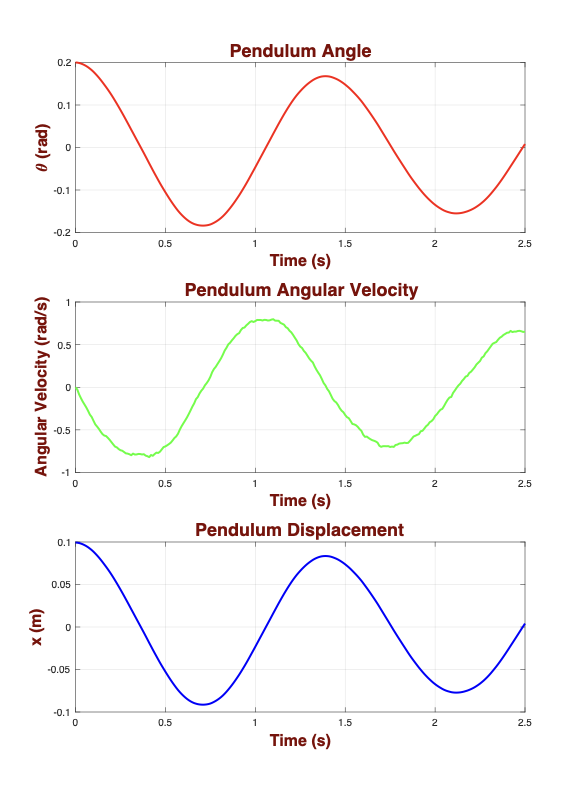
\includegraphics[width=0.8\linewidth]{Figures//Part3/PendulumMotion.png}
    \vspace{-20pt}
    \caption{Pendulum true position, angular velocity, and position, including the process noise.}
    \label{fig:enter-label}
\end{figure}

\texttt{\tiny [Code: Non-linear KF/ex12\_Pendulum\_background.m]}

\end{columns}
\end{frame}


%%%%%%%%%%%%%%%%%%%%%%%%%%%%%%%%%%%%%%%%%%%%%%
\begin{frame}{Example 12 - Estimating the Pendulum Angle: Example Summary}
The following figures compare the true, measured, and estimated pendulum angle and angular velocity for 51 measurements.
\begin{columns}
\column{0.5\textwidth}
\begin{figure}
    \centering
    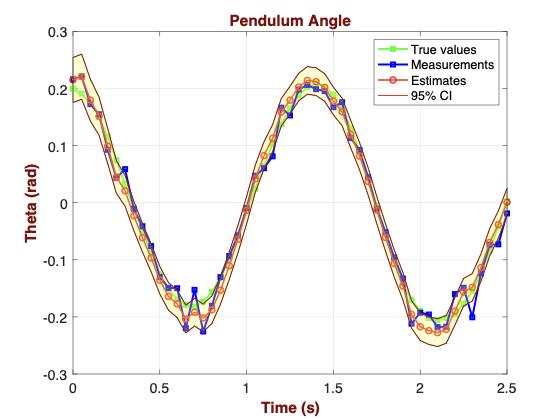
\includegraphics[width=0.95\linewidth]{Figures//Part3/Ex12_PendulumAngle.png}
    \caption{pendulum angle - true value, measured values and estimates}
\end{figure}
\column{0.5\textwidth}
\begin{figure}
    \centering
    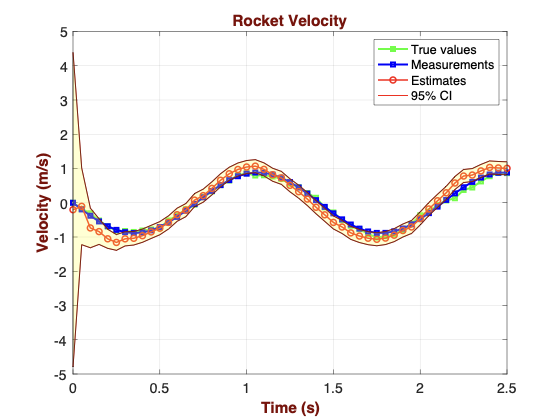
\includegraphics[width=0.95\linewidth]{Figures//Part3/Ex12_PendulumVelocity.png}
    \caption{pendulum velocity - true value, measured values and estimates.}
\end{figure}
\end{columns}

\texttt{\tiny [Code: Non-linear KF/Ex12\_EKF\_BothUncertainties.m]}
\end{frame}


%%%%%%%%%%%%%%%%%%%%%%%%%%%%%%%%%%%%%%%%%%%%%%
\subsubsection{Limitations of EKF}
\begin{frame}{Limitations of EKF--Linearization Error}
EKF performs well for many practical problems when $f(x)$ or $h(x)$ are close to
linear. However, it fails in highly non-linear regions.
\vspace{5pt}

The EKF concept is based on the linearization of the model. The EKF estimation
includes the \textbf{linearization error}. The linearization error depends on the nonlinearity
degree of the function compared to the propagated uncertainty, as shown in
the following figure.
\begin{figure}
    \centering
    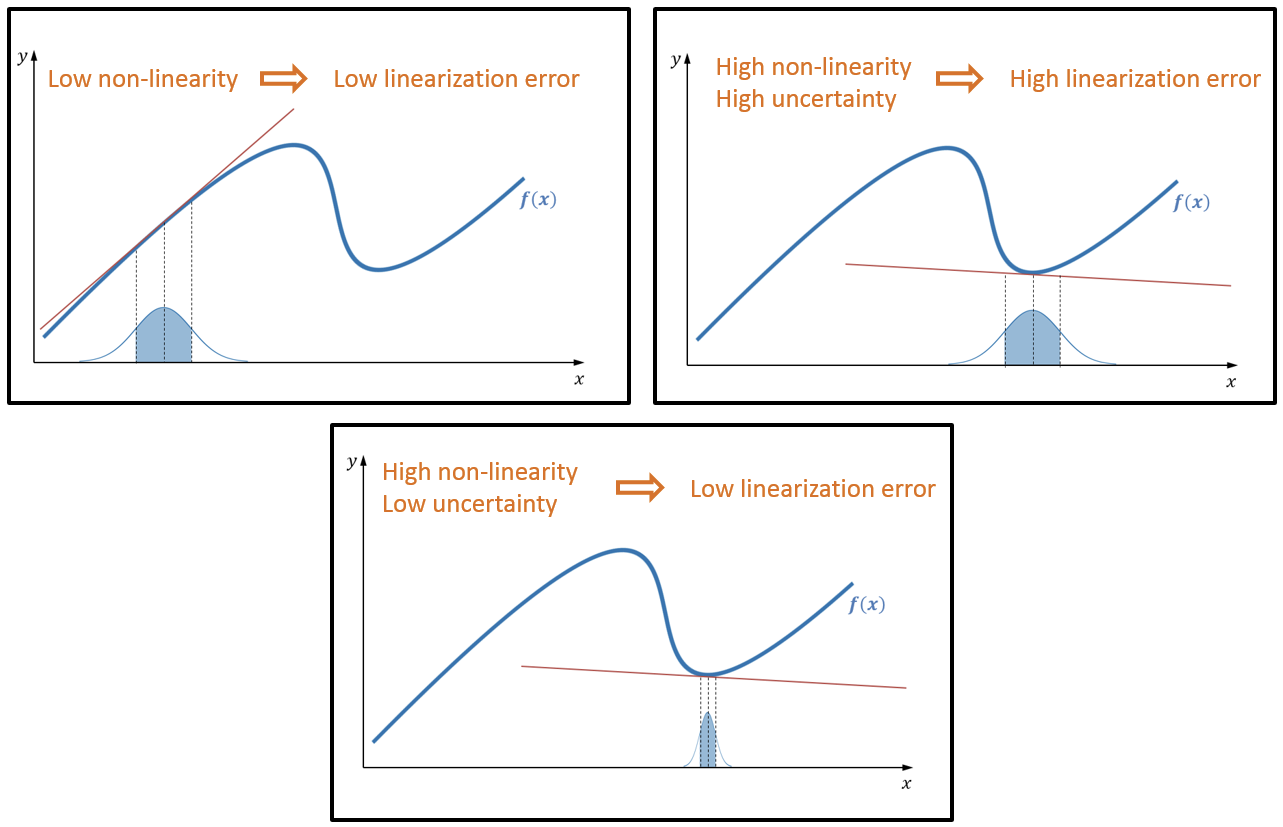
\includegraphics[width=0.7\linewidth]{Figures//Part3/LinearizarionError.png}
    \vspace{-10pt}
    \caption{LinearizarionError}
\end{figure}
\end{frame}


%%%%%%%%%%%%%%%%%%%%%%%%%%%%%%%%%%%%%%%%%%%%%%
\begin{frame}{Limitations of EKF--Linearization Error: 2D Example}
\begin{columns}
\column{0.5\textwidth}
\begin{itemize}
    \item Let us see the effect of the linearization error on polar to cartesian transformation.
    \item Assume a normally distributed random variable in polar coordinates. We want to
estimate the random variable parameters in cartesian coordinates. 
    \item A distance vector
$r$ and an angle $\theta$ describe any value in the polar coordinates. In cartesian coordinates,
the values are described by $x$ and $y$ coordinates. The dependency between $r$, $\theta$, and
$x$, $y$ is non-linear:
$$x = r\cdot\cos(\theta)$$
$$y = r\cdot\sin(\theta)$$

\item The random variable parameters \((r, \theta)\) in polar coordinates are:
\[
\mu = \begin{pmatrix}
1 & \frac{\pi}{2}
\end{pmatrix}, \quad
\sigma = \begin{pmatrix}
0.05 & 0.5
\end{pmatrix}
\]
\end{itemize}
\column{0.5\textwidth}
\begin{figure}
    \centering
    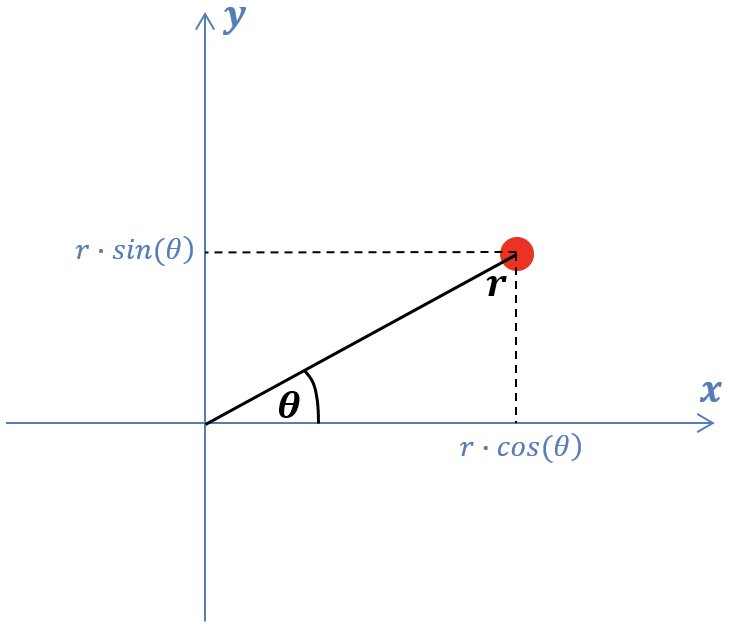
\includegraphics[width=0.6\linewidth]{Figures//Part3/2DExample_LinearizationError.png}
    \vspace{-10pt}
    \caption{Linearization Error - 2D Example}
\end{figure}
\end{columns}
\end{frame}


%%%%%%%%%%%%%%%%%%%%%%%%%%%%%%%%%%%%%%%%%%%%%%
\begin{frame}{Limitations of EKF--Linearization Error: 2D Example}
The plot on the left describes the random samples of the random variable in polar
coordinates. The right plot describes the random samples of the random variable in
cartesian coordinates after the transformation.

The ellipses on the plots represent the covariance of the random variable with 65\% confidence interval.
\begin{figure}
    \centering
    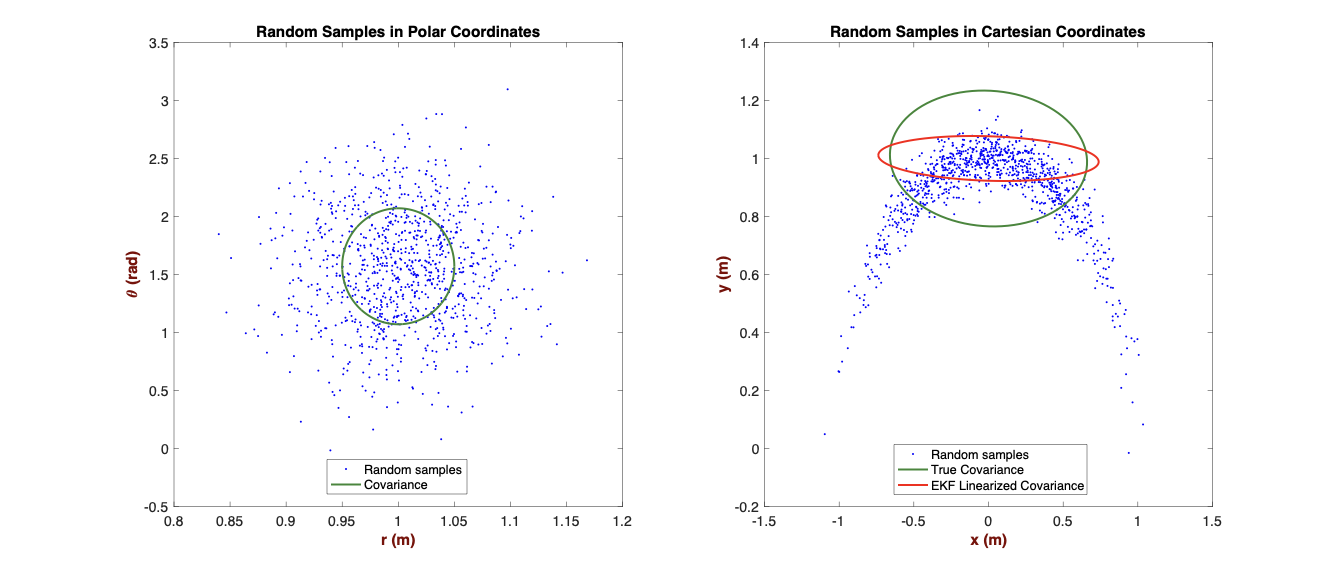
\includegraphics[width=0.7\linewidth]{Figures//Part3/LinearizationError_2D_Demo.png}
    \vspace{-10pt}
    \caption{EKF linearized covariance}
\end{figure}

We can see a significant difference between actual and EKF linearized covariance.
The EKF linearized covariance includes a high linearization error.
\vspace{5pt}

The EKF yields a wrong estimation. The EKF estimation uncertainty is also relatively
low (the error ellipse is relatively narrow). The EKF is overconfident while making a wrong
estimate!

\texttt{\tiny [Code: Non-linear KF/LinearizationError\_Polar2Cartisian.m]}
\end{frame}
%%%%%%%%%%%%%%%%%%%%%%%%%%%%%%%%%%%%%%%%%%%%%%
\begin{frame}{Limitations of EKF--Linearization Error: 2D Example - Making a case for UKF}
\textbf{\textcolor{red}{TODO-Update this slide with own figure.}}

A common alternative to the Extended Kalman Filter is the Unscented Kalman
Filter. The following plot compares EKF and UKF linearized covariance for the same example.

\begin{figure}
    \centering
    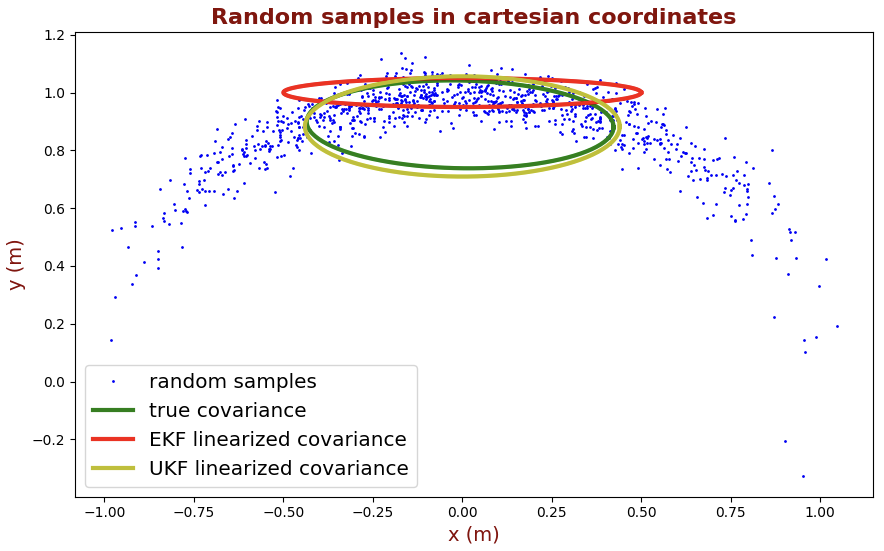
\includegraphics[width=0.5\linewidth]{Figures//Part3/EKF_vs_UKF_LinearizationError.png}
    \caption{EKF vs. UKF linearized covariance.}
\end{figure}

Observe that the UKF linearized covariance is much closer to the actual covariance
than the EKF linearized covariance.
\end{frame}


%%%%%%%%%%%%%%%%%%%%%%%%%%%%%%%%%%%%%%%%%%%%%%
\subsection{Unscented Kalman Filter (UKF)}
\begin{frame}{Unscented Kalman Filter (UKF)---Motivation}
\begin{itemize}
    \item When the State Transition model $f(x)$ and
Observation Model $h(x)$ are close to linear, the EKF performance is satisfying.
    \item However, when $f(x)$ or $h(x)$ models are highly non-linear, the linearization error can cause estimations that are significantly different from the true value of the state and estimation uncertainties that don’t capture the true uncertainties in the state.

    \item The Unscented Kalman Filter is an alternative approach to linearization. While \textcolor{blue}{Extended Kalman Filter} treats the non-linearity using \textcolor{blue}{analytical linearization}, the \textcolor{orange}{Unscented Kalman Filter} performs Unscented Transform (UT)---\textcolor{orange}{statistical linearization}.

    \item Jeffrey Uhlmann initially proposed the unscented transform (UT) as a component of his PhD thesis; however, it is predominantly known from~\cite{julier1997new}.
\end{itemize}

\end{frame}

%%%%%%%%%%%%%%%%%%%%%%%%%%%%%%%%%%%%%%%%%%%%%%
\subsubsection{The Unscented Transform (UT)}
\begin{frame}{The Unscented Transform (UT)}
\textbf{Unscented Transform:} The Unscented Transform is a method for calculating the statistics of a random
variable that undergoes a non-linear transformation.
The Unscented Transform includes three steps:
\begin{itemize}
    \item \textbf{Step 1} - Select a set of points from the input distribution. The points are selected according to a specific, deterministic algorithm.

    \item \textbf{Step 2} - Propagate each selected point through the non-linear function, producing a new set of points belonging to the output distribution.

    \item \textbf{Step 3} - Compute sigma points weights.

    \item \textbf{Step 4} - Approximate the sample mean and covariance of the output distribution using the propagated set of points and carefully chosen weights.
\end{itemize}
\end{frame}

%%%%%%%%%%%%%%%%%%%%%%%%%%%%%%%%%%%%%%%%%%%%%%
\begin{frame}{The Unscented Transform (UT): Step 1 – Sigma Points Selection}
\begin{columns}
\column{0.5\textwidth}
\vspace{-30pt}

\begin{itemize}
    \item The set of sigma points includes the mean and a certain number of points located at a certain distance away from the mean.
\end{itemize}
\textbf{Number of selected points:}
\begin{itemize}
    \item The number of selected points depends on the input distribution. 

    \item The $N$--dimensional random variable is approximated by $2N+1$ points. For a one-dimensional distribution ($N = 1$), the number of points is 3. For a two-dimensional distribution ($N = 2$), the number of points is 5.
\end{itemize}
\textbf{Selected points location:}
\begin{itemize}
 \item The first point is the mean of the input distribution:
\[ \mathcal{X}^{(0)}_{n,n} = \hat{\mathbf{x}}_{n,n}\]

The superscript in parentheses of \(\mathcal{X}^{(0)}_{n,n}\) is a sigma point number.
\end{itemize}
\column{0.5\textwidth}
\begin{itemize}
    \item The other points are located at a certain \textbf{statistical distance} from the mean, expressed in terms of standard deviation or sigma ($\sigma$). For this reason, the selected points are called the Sigma Points, and the Unscentenced Transform is sometimes called the Sigma point transform.
    \item The other sigma points location is:
\end{itemize}    
    \[
    \mathcal{X}^{(i)}_{n,n} \!=\! \hat{\mathbf{x}}_{n,n} + \left(\sqrt{(N + \kappa) \mathbf{P}_{n,n}}\right)_i, \quad i = 1, \cdots ,N
    \]
    \[
    \mathcal{X}^{(i)}_{n,n} \!=\! \hat{\mathbf{x}}_{n,n} - \left(\!\sqrt{(N + \kappa) \mathbf{P}_{n,n}}\right)_{i-N}, i \!=\! N + 1,\cdots, 2N
    \]
\vspace{-5pt}    
\begin{itemize}
    \item \(N\) is the number of dimensions
    \item \(\kappa\) is a tuning parameter
    \item \(\sqrt{(N + \kappa) \mathbf{P}_{n,n}}_i\) is the \(i\)-th row or column of the matrix square root of \(\sqrt{(N + \kappa) \mathbf{P}_{n,n}}\)
\end{itemize}
For Gaussian distribution, the rule of thumb is to set: \(N + \kappa = 3\). The sigma points should be chosen so that they capture the most important statistical properties of the prior random variable \(\hat{\mathbf{x}}\).
\end{columns}
\end{frame}

%%%%%%%%%%%%%%%%%%%%%%%%%%%%%%%%%%%%%%%%%%%%%%
\begin{frame}{The Unscented Transform (UT): Step 1 – Sigma Points Selection}
\textcolor{blue}{Note: In “Kalman Filter language,” the mean of the input distribution is the current estimate \(\hat{\mathbf{x}}_{n,n}\), and the uncertainty of the input distribution is represented by the covariance matrix of the current estimate \(\mathbf{P}_{n,n}\). The main diagonal of the covariance matrix includes variances for each dimension \((\sigma_{xx}, \sigma_{yy})\).}
\begin{columns}
\column{0.6\textwidth}

\textbf{Example: One-dimensional random variable}
Assume a zero-mean normally distributed one-dimensional random variable with a
standard deviation of 2: \(\hat{x}_{n,n} = 0\), \(p_{n,n} = 2\)
\begin{itemize}
    \item The number of dimensions: \(N = 1\)
    \item The number of sigma points: \(2N + 1 = 3\)
    \item Set: \(N + \kappa = 3\)
    \item The first point is the mean of the input distribution: \(\mathbf{X}^{(0)}_{n,n} = 0\)
    \item The second point: \(\mathbf{X}^{(1)}_{n,n} = \hat{x}_{n,n} + \sqrt{(N + \kappa)P_{n,n}}_1 = 0 + \sqrt{3 \cdot 2^2} = 3.46\)
    \item The third point: \(\mathbf{X}^{(2)}_{n,n} = \hat{x}_{n,n} - \sqrt{(N + \kappa)P_{n,n}}_2 = 0 - \sqrt{3 \cdot 2^2} = -3.46\)
\end{itemize}

\column{0.4\textwidth}
The Unscented Transform sigma points are not necessarily on the standard deviation
boundaries.
\begin{figure}
    \centering
    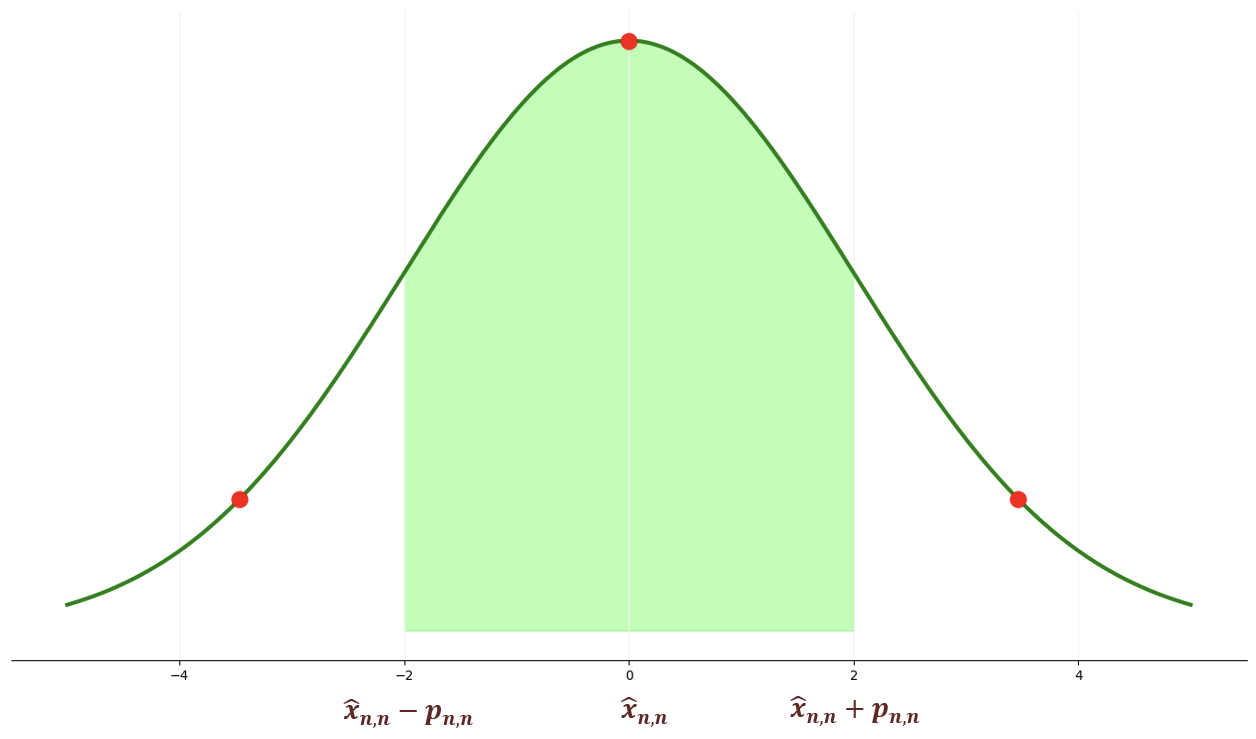
\includegraphics[width=0.95\linewidth]{Figures//Part3/1DSigmaPoints_examples.png}
    \caption{1D Sigma Points}
\end{figure}
\end{columns}
\end{frame}

%%%%%%%%%%%%%%%%%%%%%%%%%%%%%%%%%%%%%%%%%%%%%%
\begin{frame}{The Unscented Transform (UT): Step 1 – Sigma Points Selection}
\begin{columns}
\column{0.5\textwidth}
\textbf{Example: Two-dimensional random variable:} Consider the earlier example with polar \((r, \theta)\) to cartesian transformation. 
\[
\mathbf{x}_{n,n} =
\begin{bmatrix}
1 \\
\pi/2
\end{bmatrix}
=
\begin{bmatrix}
1 \\
1.57
\end{bmatrix}
\]

\[
\mathbf{P}_{n,n} =
\begin{bmatrix}
0.05^2 & 0 \\
0 & 0.5^2
\end{bmatrix}
=
\begin{bmatrix}
0.0025 & 0 \\
0 & 0.25
\end{bmatrix}
\]

Finding the sigma points:
\begin{itemize}
    \item The number of dimensions: \(N = 2\)
    \item The number of sigma points: \(2N + 1 = 5\)
    \item Set: \(N + \kappa = 3\)
    \item The first point is the mean of the input distribution: \(\mathcal{X}^{(0)}_{n,n} =
    \begin{bmatrix}
    1 \\
    1.57
    \end{bmatrix}\)
    \item To find the other points, we should compute: \(\sqrt{(N + \kappa)\mathbf{P}_{n,n}}\)
\end{itemize}
\[
\sqrt{(N + \kappa)\mathbf{P}_{n,n}} \!=\! \sqrt{3\! \begin{bmatrix}
0.0025 & 0 \\
0 & 0.25
\end{bmatrix}}
\!=\! \sqrt{\begin{bmatrix}
0.0075 & 0 \\
0 & 0.75
\end{bmatrix}}
\]
\column{0.5\textwidth}
\begin{itemize}
    \item We need to find the square root of the matrix. Luckily, the covariance matrix is positive and semi-definite; therefore, we can use Cholesky decomposition to find the square root.
    $$(N+\kappa)\mathbf{P}_{n,n}$$

    \item L is a lower triangular matrix, which can be computed in Matlab as L = chol (P)’

    \[
    \mathbf{L} =
    \begin{bmatrix}
    0.0866 & 0 \\
    0 & 0.866
    \end{bmatrix}
    \]
\end{itemize}
\end{columns}
\end{frame}

%%%%%%%%%%%%%%%%%%%%%%%%%%%%%%%%%%%%%%%%%%%%%%
\begin{frame}{The Unscented Transform (UT): Step 1 – Sigma Points Selection}
The second point: \(\mathcal{X}^{(1)}_{n,n} = \hat{\mathbf{x}}_{n,n} + \left(\sqrt{(N + \kappa)\mathbf{P}_{n,n}}\right)_1 = 
\begin{bmatrix}
1 \\
1.57
\end{bmatrix}
+
\begin{bmatrix}
0.0866 \\
0
\end{bmatrix}
=
\begin{bmatrix}
1.0866 \\
1.57
\end{bmatrix}
\)
%\vspace{10pt}

The third point: \(\mathcal{X}^{(2)}_{n,n} = \hat{\mathbf{x}}_{n,n} + \left(\sqrt{(N + \kappa)\mathbf{P}_{n,n}}\right)_2 = 
\begin{bmatrix}
1 \\
1.57
\end{bmatrix}
+
\begin{bmatrix}
0 \\
0.866
\end{bmatrix}
=
\begin{bmatrix}
1 \\
2.436
\end{bmatrix}
\)
%\vspace{10pt}

The fourth point: \(\mathcal{X}^{(3)}_{n,n} = \hat{\mathbf{x}}_{n,n} - \left(\sqrt{(N + \kappa)\mathbf{P}_{n,n}}\right)_1 = 
\begin{bmatrix}
1 \\
1.57
\end{bmatrix}
-
\begin{bmatrix}
0.0866 \\
0
\end{bmatrix}
=
\begin{bmatrix}
0.9134 \\
1.57
\end{bmatrix}
\)
%\vspace{10pt}

The fifth point: \(\mathcal{X}^{(4)}_{n,n} = \hat{\mathbf{x}}_{n,n} - \left(\sqrt{(N + \kappa)\mathbf{P}_{n,n}}\right)_2 = 
\begin{bmatrix}
1 \\
1.57
\end{bmatrix}
-
\begin{bmatrix}
0 \\
0.866
\end{bmatrix}
=
\begin{bmatrix}
1 \\
0.704
\end{bmatrix}
\)

The following figure describes the covariance ellipse of the random variable PDF
with sigma points (red circles).
\begin{figure}
    \centering
    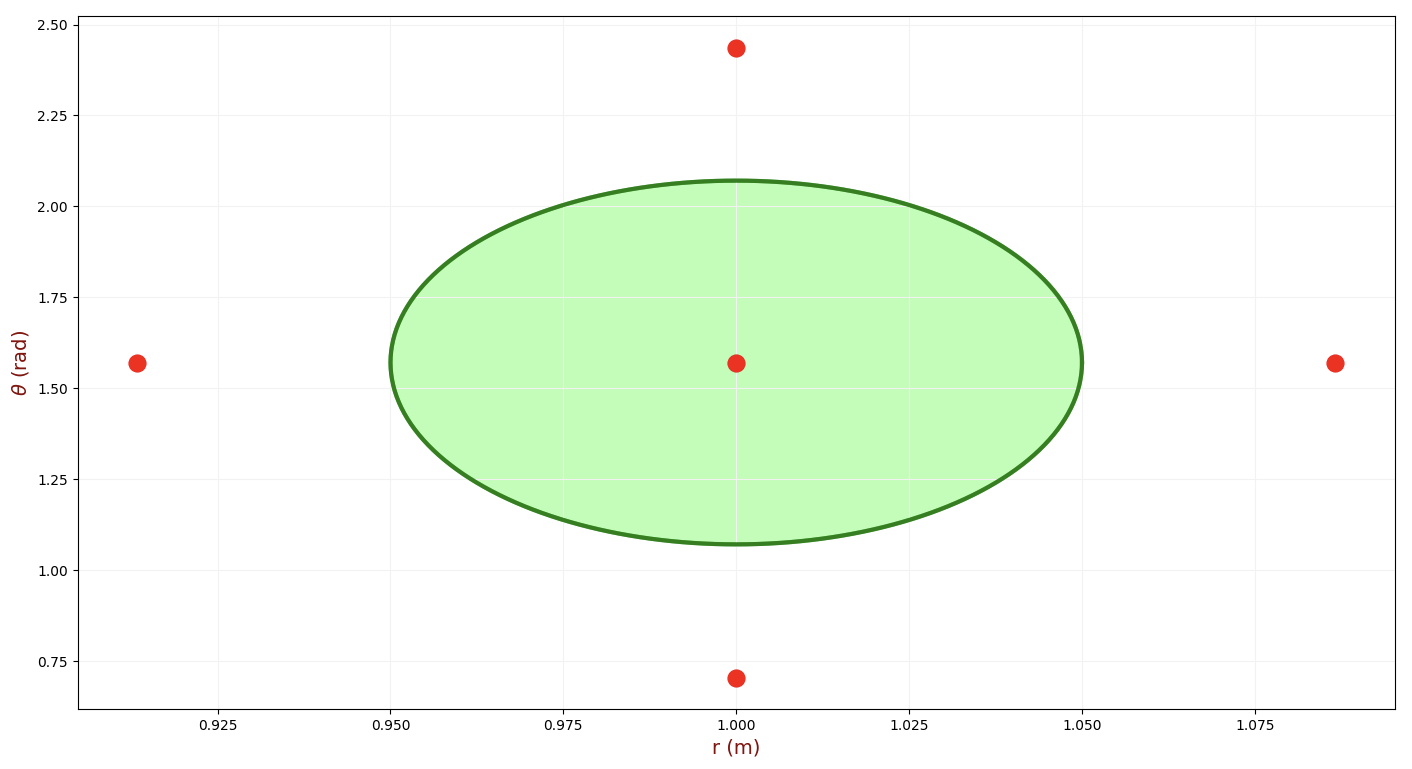
\includegraphics[width=0.5\linewidth]{Figures//Part3/2DSigmaPoints_Example.png}
    \vspace{-10pt}
    \caption{2D RV Sigma Points}
    \vspace{-10pt}
\end{figure}
The Unscented Transform sigma points are not necessarily on the covariance ellipse
boundaries.
\end{frame}


%%%%%%%%%%%%%%%%%%%%%%%%%%%%%%%%%%%%%%%%%%%%%%
\begin{frame}{The Unscented Transform (UT): Step 2 – Points Propagation}
Propagate each selected point through the non-linear function, producing a new set of points belonging to the output distribution.
\begin{columns}
\column{0.5\textwidth}
\textbf{Example: one-dimensional random variable (continued)}
The non-linear function is:
\[
f(x) = \sin(2x)\sin(0.3x) + 2x
\]

\[
\mathcal{X}_{n+1,n} = f(\mathcal{X}_{n,n})
\]

The propagated (or transformed) sigma points:
\[
\mathcal{X}^{(0)}_{n+1,n} = \sin(2 \cdot 0)\sin(0.3 \cdot 0) + 2 \cdot 0 = 0
\]

\[
\mathcal{X}^{(1)}_{n+1,n} = \sin(2 \cdot 3.46)\sin(0.3 \cdot 3.46) + 2 \cdot 3.46 = 7.45
\]

\begin{align*}
  \mathcal{X}^{(2)}_{n+1,n} & = \sin(2 \cdot (-3.46))\sin(0.3 \cdot (-3.46)) \\ & + 2 \cdot (-3.46) = -6.41  
\end{align*}

\column{0.5\textwidth}
\begin{figure}
    \centering
    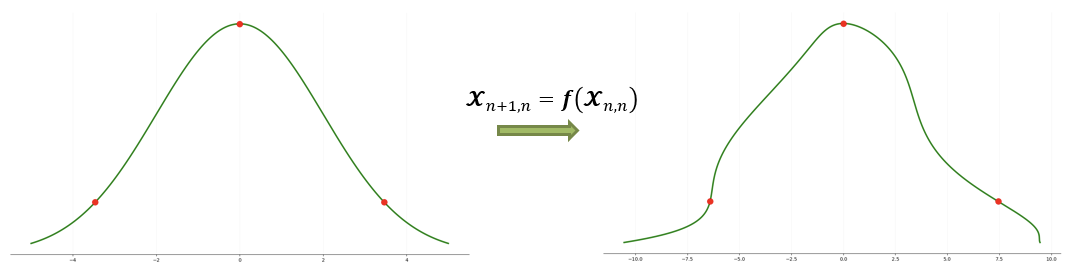
\includegraphics[width=0.95\linewidth]{Figures//Part3/1DSigmaPointPropagation.png}
    \caption{1D RV Sigma Points propagation.}
\end{figure}
\begin{itemize}
    \item The green line on the left plot is the PDF of the input random variable. The red
circles on the left plot are the sigma points ($\mathcal{X}_{n,n}$) of the input random variable.
\item The green line on the right plot is the PDF of the input random variable after the
non-linear transformation. The red circles on the right plot are the sigma points
after the non-linear transformation ($\mathcal{X}_{n+1,n}$).
\end{itemize}
\end{columns}
\end{frame}


%%%%%%%%%%%%%%%%%%%%%%%%%%%%%%%%%%%%%%%%%%%%%%
\begin{frame}{The Unscented Transform (UT): Step 2 – Points Propagation}



\begin{columns}
\column{0.5\textwidth}
Example: two-dimensional random variable (continued)
The non-linear function is:
\[
\begin{bmatrix}
x \\
y
\end{bmatrix}
=
\begin{bmatrix}
r \cdot \cos(\theta) \\
r \cdot \sin(\theta)
\end{bmatrix}
\]
\[
\mathbf{\mathcal{X}}_{n+1,n} = \mathbf{f}(\mathbf{\mathcal{X}}_{n,n})
\]

The propagated (or transformed) sigma points:
\[
\mathbf{\mathcal{X}}^{(0)}_{n+1,n} = \mathbf{f}(\mathbf{\mathcal{X}}^{(0)}_{n,n}) =
\begin{bmatrix}
1 \cdot \cos\left(\frac{\pi}{2}\right) \\
1 \cdot \sin\left(\frac{\pi}{2}\right)
\end{bmatrix}
\!=\!
\begin{bmatrix}
0 \\
1
\end{bmatrix}
\]
\[
\mathbf{\mathcal{X}}^{(1)}_{n+1,n} \!=\! \mathbf{f}(\mathbf{\mathcal{X}}^{(1)}_{n,n}) \!=\!
\begin{bmatrix}
1.0866 \cdot \cos\left(\frac{\pi}{2}\right) \\
1.0866 \cdot \sin\left(\frac{\pi}{2}\right)
\end{bmatrix}
\!=\!
\begin{bmatrix}
0 \\
1.0866
\end{bmatrix}
\]
\[
\mathbf{\mathcal{X}}^{(2)}_{n+1,n} \!=\! \mathbf{f}(\mathbf{\mathcal{X}}^{(2)}_{n,n}) \!=\!
\begin{bmatrix}
1 \cdot \cos(2.436) \\
1 \cdot \sin(2.436)
\end{bmatrix}
\!=\!
\begin{bmatrix}
-0.762 \\
0.648
\end{bmatrix}
\]
\[
\mathbf{\mathcal{X}}^{(3)}_{n+1,n} \!=\! \mathbf{f}(\mathbf{\mathcal{X}}^{(3)}_{n,n}) \!=\!
\begin{bmatrix}
0.9134 \cdot \cos\left(\frac{\pi}{2}\right) \\
0.9134 \cdot \sin\left(\frac{\pi}{2}\right)
\end{bmatrix}
\!=\!
\begin{bmatrix}
0 \\
0.9134
\end{bmatrix}
\]
\[
\mathbf{\mathcal{X}}^{(4)}_{n+1,n} \!=\! \mathbf{f}(\mathbf{\mathcal{X}}^{(4)}_{n,n}) \!=\!
\begin{bmatrix}
1 \cdot \cos(0.704) \\
1 \cdot \sin(0.704)
\end{bmatrix}
\!=\!
\begin{bmatrix}
0.762 \\
0.648
\end{bmatrix}
\]
\column{0.5\textwidth}
\begin{figure}
    \centering
    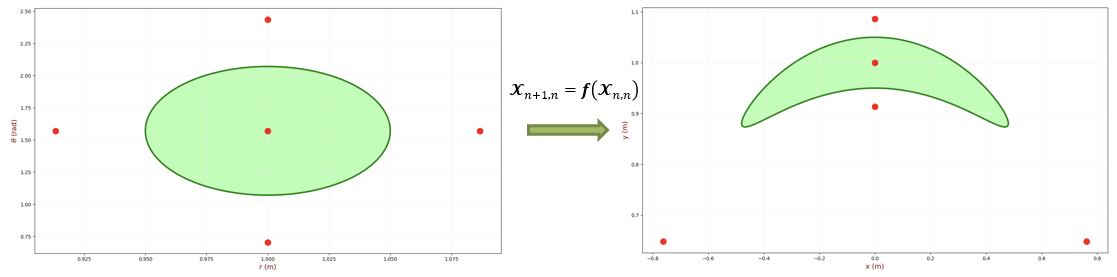
\includegraphics[width=0.95\linewidth]{Figures//Part3/2DSigmaPointsPropagation.png}
    \caption{2D RV Sigma Points propagation.}
\end{figure}
\begin{itemize}
    \item The green shape on the left plot is the covariance ellipse of the input random variable. The red circles on the left plot are the sigma points ($\mathcal{X}_{n,n}$) of the input random variable.
    \item The green shape on the right plot is the covariance ellipse of the input random variable after the non-linear transformation. The red circles on the right plot are the sigma points after the non-linear transformation ($\mathcal{X}_{n+1,n}$).
\end{itemize}

\end{columns}
\end{frame}


%%%%%%%%%%%%%%%%%%%%%%%%%%%%%%%%%%%%%%%%%%%%%%
\begin{frame}{The Unscented Transform (UT): Step 3 \& 4}

\textcolor{blue}{\textbf{Step 3 – compute sigma points weights}}

We should compute two weights:
\begin{itemize}
    \item \(w_0\)---weight of the first sigma point \(\mathbf{\mathcal{X}}^{(0)}_{n,n}\)

    \[
    w_0 = \frac{\kappa}{N + \kappa}
    \]
    
    \item \(w_i\)---weight of the other sigma points \(\mathbf{\mathcal{X}}^{(i)}_{n,n}\), \(i > 0\)

    \[
    w_i = \frac{1}{2(N + \kappa)}, \quad i > 0
    \]
\end{itemize}

\textcolor{blue}{\textbf{The Unscented Transform (UT): Step 4 - approximate the mean and covariance of the output
distribution}:} In this step, we approximate the sample mean and covariance of the output distribution using the propagated set of points and carefully chosen weights.

\begin{itemize}
    \item The mean of the output distribution:
\[
\hat{x}_{n+1,n} = \sum_{i=0}^{2N} w_i \mathbf{\mathcal{X}}^{(i)}_{n+1,n}
\]

\item The covariance of the output is also computed with weights:
\[
\mathbf{P}_{n+1,n} = \sum_{i=0}^{2N} w_i \left( \mathbf{\mathcal{X}}^{(i)}_{n+1,n} - \hat{x}_{n+1,n} \right) \left( \mathbf{\mathcal{X}}^{(i)}_{n+1,n} - \hat{x}_{n+1,n} \right)^T
\]
\end{itemize}




\end{frame}


%%%%%%%%%%%%%%%%%%%%%%%%%%%%%%%%%%%%%%%%%%%%%%
\begin{frame}{The Unscented Transform (UT): Step 4 - approximate the mean and covariance of the output
distribution (Examples)}
\begin{columns}
\column{0.5\textwidth}
\textbf{Example: one-dimensional random variable}

\textbf{Weights computation:}
\begin{itemize}
    \item The number of dimensions: \(N = 1\)
    \item \(N + \kappa = 3\), \(\kappa = 2\)
\end{itemize}
\vspace{-5pt}
\[
w_0 = \frac{\kappa}{N + \kappa} = \frac{2}{3}
\]
\[
w_i = \frac{1}{2(N + \kappa)} = \frac{1}{2 \cdot 3} = \frac{1}{6}
\]
\vspace{-5pt}

\textbf{Mean computation:}
\vspace{-17pt}

\begin{align*}
\hat{x}_{n+1,n} & = \sum_{i=0}^{2N} w_i \mathcal{X}^{(i)}_{n+1,n} \\ &= \frac{2}{3} \cdot 0 + \frac{1}{6} \cdot 7.45 + \frac{1}{6} \cdot (-6.42) = 0.17 
\end{align*}
\vspace{-10pt}

\textbf{Covariance computation (variance in 1D):}
\vspace{-17pt}

\begin{align*}
\mathbf{P}_{n+1,n} & = \sum_{i=0}^{2N} w_i \left( \mathcal{X}^{(i)}_{n+1,n} - \hat{x}_{n+1,n} \right) \left( \mathcal{X}^{(i)}_{n+1,n} - \hat{x}_{n+1,n} \right)^T  \\
& =\frac{2}{3} \cdot (0 - 0.17)^2 + \frac{1}{6} \cdot (7.45 - 0.17)^2 +\\ 
& \frac{1}{6} \cdot (-6.42 - 0.17)^2 = 16.06
\end{align*}

\column{0.5\textwidth}
The following plot depicts the output random variable after the Unscented Transform.
\begin{figure}
    \centering
    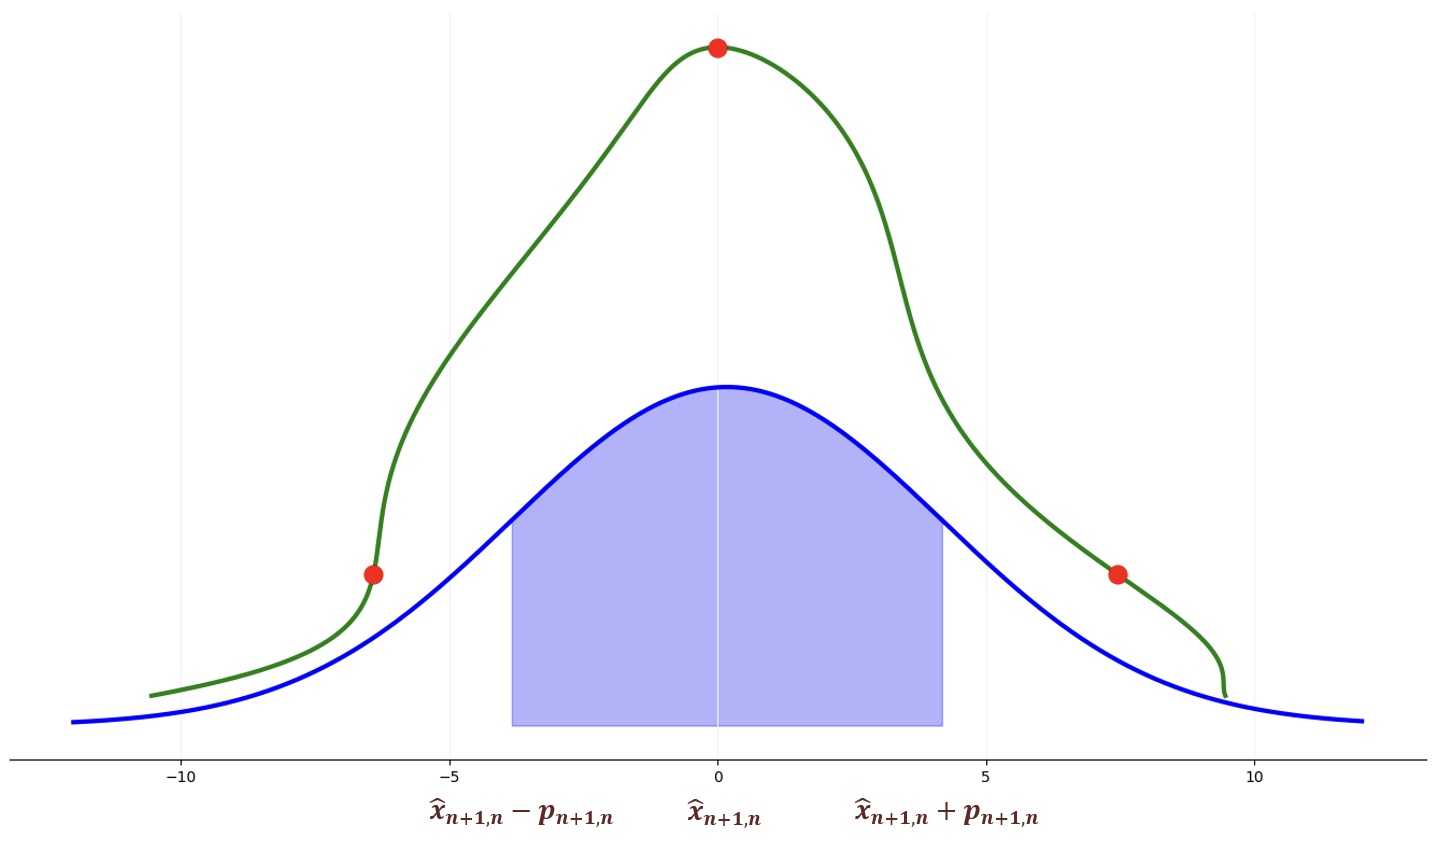
\includegraphics[width=0.95\linewidth]{Figures//Part3/1DUncentedTransform.png}
    \caption{1D RV Unscented Transform}

    \begin{itemize}
        \item The green line is the PDF of the input random variable after non-linear transformation. The red circles are the sigma points after the non-linear transformation ($\mathcal{X}_{n+1,n}$).
        \item The blue line is the PDF of the output random variable after the Unscented Transform.
    \end{itemize}
\end{figure}
\end{columns}
\end{frame}


%%%%%%%%%%%%%%%%%%%%%%%%%%%%%%%%%%%%%%%%%%%%%%
\begin{frame}{The Unscented Transform (UT): Step 4 - approximate the mean and covariance of the output distribution}
\begin{columns}
\column{0.4\textwidth}
\textbf{Example: two-dimensional random variable  (continued)}
\textbf{Weights computation:}
\begin{itemize}
    \item The number of dimensions: \(N = 2\)
    \item \(N + \kappa = 3\)
    \item \(\kappa = 1\)
\end{itemize}

\[
w_0 = \frac{\kappa}{N + \kappa} = \frac{1}{3}
\]

\[
w_i = \frac{1}{2(N + \kappa)} = \frac{1}{2 \cdot 3} = \frac{1}{6}
\]

\textbf{Mean computation:}
\begin{align*}
\hat{x}_{n+1,n} & = \sum_{i=0}^{2N} w_i \mathcal{X}^{(i)}_{n+1,n} = \frac{1}{3}
\begin{bmatrix}
0 \\
1
\end{bmatrix}
+ \frac{1}{6}
\begin{bmatrix}
0 \\
1.0866
\end{bmatrix} \\
& + \frac{1}{6}
\begin{bmatrix}
-0.762 \\
0.648
\end{bmatrix}
+ \frac{1}{6}
\begin{bmatrix}
0 \\
0.913
\end{bmatrix}
+ \frac{1}{6}
\begin{bmatrix}
0.762 \\
0.648
\end{bmatrix} \\
& =
\begin{bmatrix}
0 \\
0.8826
\end{bmatrix}    
\end{align*}

\column{0.58\textwidth}
\begin{align*}
& \mathbf{P}_{n+1,n}  \\ & = \sum_{i=0}^{2N} w_i \left( \mathcal{X}^{(i)}_{n+1,n} - \hat{x}_{n+1,n} \right) \left( \mathcal{X}^{(i)}_{n+1,n} - \hat{x}_{n+1,n} \right)^T \\
& = \frac{1}{3}
\left(
\begin{bmatrix}
0 \\
1
\end{bmatrix}
-
\begin{bmatrix}
0 \\
0.8826
\end{bmatrix}
\right)
\left(
\begin{bmatrix}
0 \\
1
\end{bmatrix}
-
\begin{bmatrix}
0 \\
0.8826
\end{bmatrix}
\right)^T \\
& \!+\! \frac{1}{6}\!
\left(
\begin{bmatrix}
0 \\
1.0866
\end{bmatrix}
\!-\!
\begin{bmatrix}
0 \\
0.8826
\end{bmatrix}
\right)\!\!
\left(\!
\begin{bmatrix}
0 \\
1.0866
\end{bmatrix}
\!-\!
\begin{bmatrix}
0 \\
0.8826
\end{bmatrix}\!
\right)^T \\
& \!+\! \frac{1}{6}\!
\left(\!
\begin{bmatrix}
-0.762 \\
0.648
\end{bmatrix}
\!-\!
\begin{bmatrix}
0 \\
0.8826
\end{bmatrix}
\right)\!\!
\left(\!
\begin{bmatrix}
-0.762 \\
0.648
\end{bmatrix}
\!-\!
\begin{bmatrix}
0 \\
0.8826
\end{bmatrix}\!
\right)^T \\
& \!+\! \frac{1}{6}\!
\left(
\begin{bmatrix}
0 \\
0.913
\end{bmatrix}
-
\begin{bmatrix}
0 \\
0.8826
\end{bmatrix}
\right)\!\!
\left(\!
\begin{bmatrix}
0 \\
0.913
\end{bmatrix}
-
\begin{bmatrix}
0 \\
0.8826
\end{bmatrix}
\right)^T\\
& \!+\! \frac{1}{6}\!
\left(\!
\begin{bmatrix}
0.762 \\
0.648
\end{bmatrix}
\!-\!
\begin{bmatrix}
0 \\
0.8826
\end{bmatrix}
\right)\!\!
\left(\!
\begin{bmatrix}
0.762 \\
0.648
\end{bmatrix}
\!-\!
\begin{bmatrix}
0 \\
0.8826
\end{bmatrix}\!
\right)^T \\
& =
\begin{bmatrix}
0.193 & 0 \\
0 & 0.03
\end{bmatrix}   
\end{align*}
\end{columns}
\end{frame}


%%%%%%%%%%%%%%%%%%%%%%%%%%%%%%%%%%%%%%%%%%%%%%
\begin{frame}{The Unscented Transform (UT): Step 4 - approximate the mean and covariance of the output distribution}
\begin{columns}
\column{0.5\textwidth}
We can compute the mean and covariance more elegantly.

Define a matrix (container) of transformed sigma points:
\[
\mathbf{X}_{n+1,n} =
\begin{bmatrix}
\mathcal{X}^{(0)}_{n+1,n} & \mathcal{X}^{(1)}_{n+1,n} & \cdots & \mathcal{X}^{(2N)}_{n+1,n}
\end{bmatrix}
\]

Define a vector of weights:
\[
\mathbf{w} =
\begin{bmatrix}
w_0 & w_1 & \cdots & w_{2N}
\end{bmatrix}
\]

Mean computation:
\[
\hat{x}_{n+1,n} = \mathcal{X}_{n+1,n} \mathbf{w}
\]
\begin{align*}
\hat{x}_{n+1,n} & =
\begin{bmatrix}
0 & 0 & -0.762 & 0 & 0.762 \\
1 & 1.0866 & 0.648 & 0.913 & 0.648
\end{bmatrix}\\
\times &
\begin{bmatrix}
\frac{1}{3} \\
\frac{1}{6} \\
\frac{1}{6} \\
\frac{1}{6} \\
\frac{1}{6}
\end{bmatrix}
=
\begin{bmatrix}
0 \\
0.8826
\end{bmatrix}    
\end{align*}
\column{0.5\textwidth}
Covariance computation:
\begin{align*}
& \mathbf{P}_{n+1,n}  \\ & = (\mathcal{X}_{n+1,n} - \hat{x}_{n+1,n}) \cdot \text{diag}(\mathbf{w}) \cdot (\mathcal{X}_{n+1,n} - \hat{x}_{n+1,n})^T
\end{align*}
\begin{figure}
    \centering
    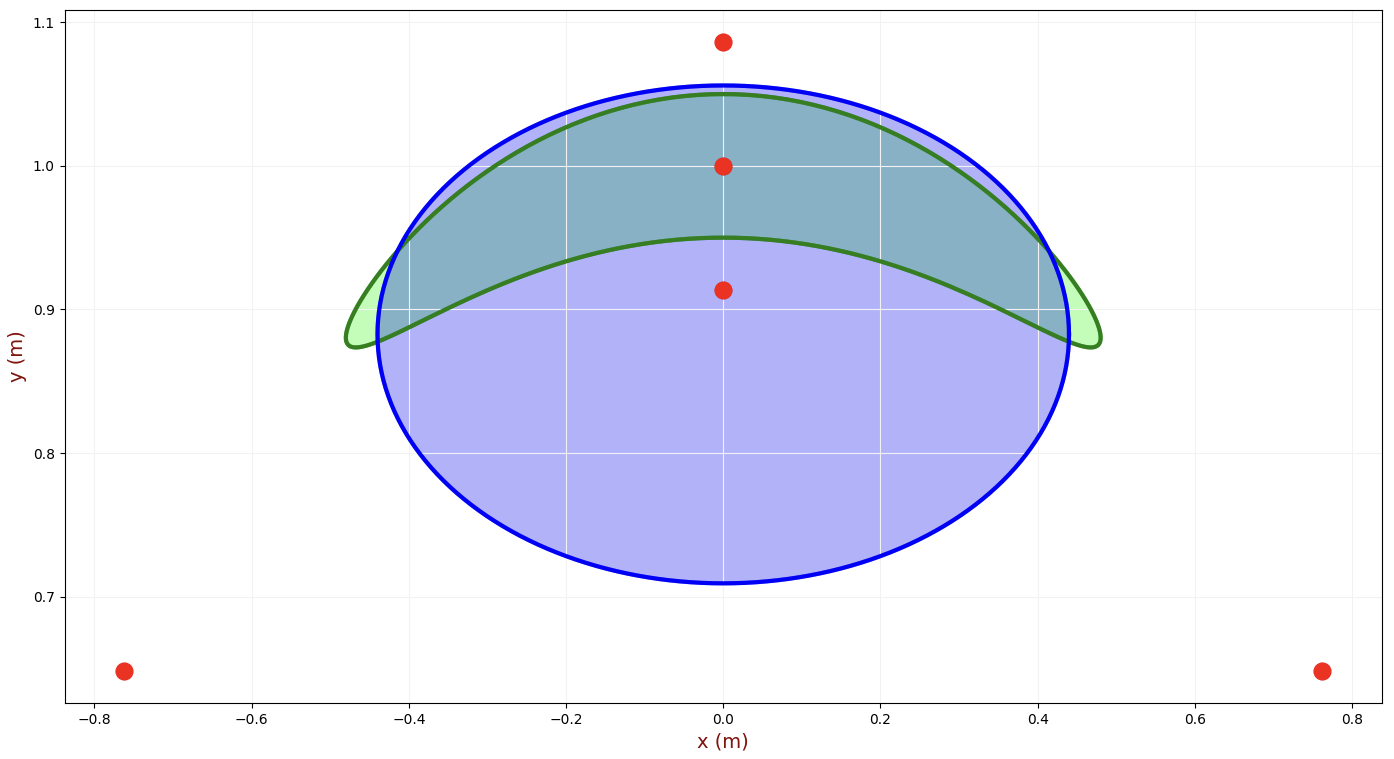
\includegraphics[width=0.5\linewidth]{Figures//Part3/2DUncentedTransform.png}
    \caption{2D RV Unscented Transform.}
\end{figure}
\begin{itemize}
    \item The green shape is the covariance ellipse of the input random variable after the non-linear transformation. The red circles on the right plot are the sigma points after the non-linear transformation ($\mathcal{X}_{n+1,n}$).

    \item The blue ellipse is the covariance ellipse of the output random variable after the Unscented Transform.
\end{itemize}
\end{columns}
\end{frame}


%%%%%%%%%%%%%%%%%%%%%%%%%%%%%%%%%%%%%%%%%%%%%%
\subsubsection{The UKF algorithm: Prediction and Update Stages}
\begin{frame}{The UKF algorithm - Prediction Stage}
UKF operates in a “predict–correct” loop, business as usual. In the prediction stage, UKF extrapolates the current estimate to the next state using the Unscented Transform:
\[
\hat{\mathbf{x}}_{n,n} \rightarrow \hat{\mathbf{x}}_{n+1,n}
\]
\[
\mathbf{P}_{n,n} \rightarrow \mathbf{P}_{n+1,n}
\]
\vspace{-14pt}
\begin{figure}
    \centering
    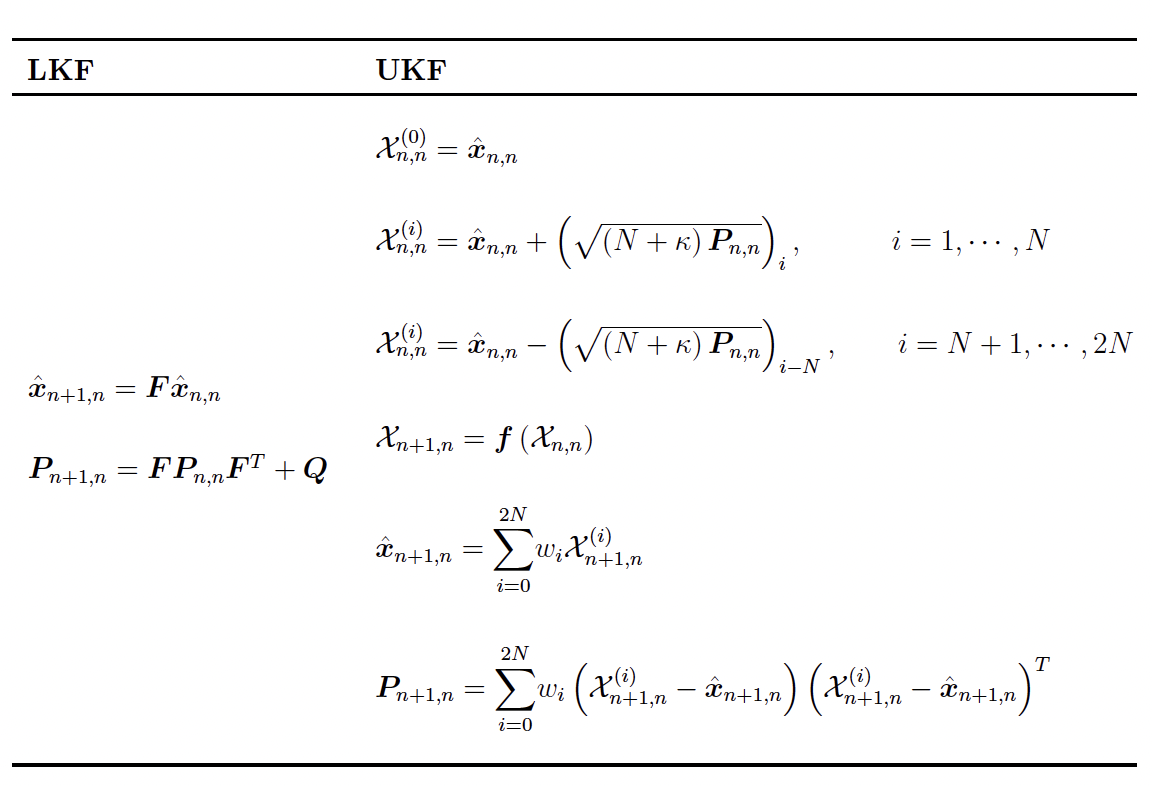
\includegraphics[width=0.75\linewidth]{Figures//Part3/UKF_PredictionStage.png}
    \vspace{-12pt}
    \caption{LKF and UKF predict stage equations.}
\end{figure}
\end{frame}


%%%%%%%%%%%%%%%%%%%%%%%%%%%%%%%%%%%%%%%%%%%%%%
\begin{frame}{The UKF algorithm - Update Stage}
Before proceeding to the update stage, 
the \textbf{statistical linear regression} concept must be understood.
\begin{columns}
\column{0.5\textwidth}
Consider a non-linear function $\mathbf{y} = g(\mathbf{x})$ evaluated at $r$ points $(\mathbf{\mathcal{X}}(i), \mathbf{\mathcal{Y}}(i))$, where $\mathbf{\mathcal{Y}}(i) = g(\mathbf{\mathcal{X}}(i))$.
Let's define:
\begin{figure}
    \centering
    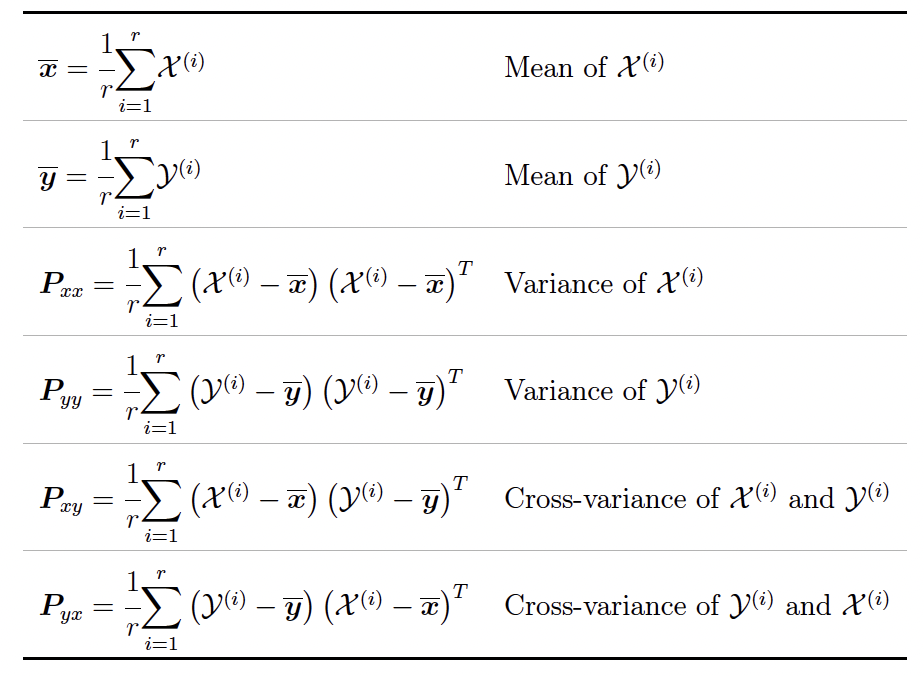
\includegraphics[width=0.9\linewidth]{Figures//Part3/StatisticalLinearRegression.png}
    \vspace{-10pt}
    \caption{Definitions}
\end{figure}
\column{0.5\textwidth}
We want to approximate the non-linear function $\mathbf{y} = g(\mathbf{x})$ by a linear function
$\mathbf{y} = \mathbf{M}\mathbf{x} + \mathbf{b}$.
The linear approximation produces linearization error. For each point $\mathbf{\mathcal{X}}^{(i)}$, the
linearization error is given by
\[
\mathbf{e}^{(i)} = \mathbf{\mathcal{Y}}^{(i)} - (\mathbf{M}\mathbf{\mathcal{X}}^{(i)} + \mathbf{b})
\]
To minimize the linearization error, we should find $\mathbf{M}$ and $\mathbf{b}$ that minimize the sum
of squared errors for all $\mathbf{\mathcal{X}}(i)$ points:
\[
\min_{\mathbf{M},\mathbf{b}} \sum_{i=1}^{r} (\mathbf{e}(i))^T \mathbf{e}(i)
\]
The solution of this minimization problem is:

$$\boxed{
\begin{aligned}
& \mathbf{M} = \mathbf{P}_{xy}^T \mathbf{P}_{xx}^{-1} = \mathbf{P}_{yx} \mathbf{P}_{xx}^{-1}\\
& \mathbf{b} = \mathbf{\Bar{z}} - \mathbf{M\Bar{x}}
\end{aligned}
}$$
{\footnotesize See proof in Appendix~F of the book.}

\end{columns}
\end{frame}

%%%%%%%%%%%%%%%%%%%%%%%%%%%%%%%%%%%%%%%%%%%%%%
\begin{frame}{The UKF algorithm - Update Stage}
\begin{columns}
\column{0.5\textwidth}
\textbf{State update:}
After a unit delay, the $\mathbf{\mathcal{X}}_{n+1,n}$ becomes $\mathbf{\mathcal{X}}_{n,n-1}$, and $\hat{\mathbf{x}}_{n+1,n}$ becomes $\hat{\mathbf{x}}_{n,n-1}$.
\vspace{5pt}

Using the Unscented Transform, transfer the state sigma points $(\mathbf{\mathcal{X}}_{n,n-1})$ to the
measurement space ($\mathbf{\mathcal{Z}}$) using the measurement function $\mathbf{h}(\mathbf{x})$:
\[
\mathbf{\mathcal{Z}}_n = \mathbf{h}(\mathbf{\mathcal{X}}_{n,n-1})
\]
\[
\mathbf{\Bar{z}}_n = \sum_{i=0}^{2N} w_i \mathbf{Z}_n^{(i)}
\]
Update estimate with measurement:
\[
\boxed{\hat{\mathbf{x}}_{n,n} = \hat{\mathbf{x}}_{n,n-1} + \mathbf{K}_n (\mathbf{z}_n - \bar{\mathbf{z}}_n)}
\]

\textbf{Kalman gain derivation:}
The Kalman Gain ($\mathbf{K}_n$) transforms the innovation ($\mathbf{z}_n - \bar{\mathbf{z}}_n$) and the measurement
covariance ($\mathbf{P}_{\mathbf{z}_n}$) from the measurement space to the system space using linearization:
\[
\text{innovation} = (\mathbf{M}\mathbf{z}_n + \mathbf{b}) - (\mathbf{M}\bar{\mathbf{z}}_n + \mathbf{b}) = \mathbf{M}(\mathbf{z}_n - \bar{\mathbf{z}}_n)
\]

\column{0.5\textwidth}
Since the Kalman Gain performs a linear transformation, it produces linearization
errors. We want to minimize the linearization errors using the statistical linear
regression method. Therefore, the Kalman gain is given by:
\[
\boxed{
\mathbf{K}_n = \mathbf{M} = \mathbf{P}_{\mathbf{x}\mathbf{z}_n} \mathbf{P}_{\mathbf{z}_n}^{-1}
}
\]
Compute the weighted variance of the measurement ($\mathbf{P}_{\mathbf{z}_n}$) and cross-covariance of
the state and the measurement ($\mathbf{P}_{\mathbf{x}\mathbf{z}_n}$):
$$
\boxed{
\begin{aligned}
\mathbf{P}_{\mathbf{z}_n} & = \sum_{i=0}^{2N} w_i \left(\mathbf{\mathcal{Z}}_n^{(i)} - \bar{\mathbf{z}}_n\right) \left(\mathbf{\mathcal{Z}}_n^{(i)} - \bar{\mathbf{z}}_n\right)^T + \mathbf{R}_n\\
\mathbf{P}_{\mathbf{x}\mathbf{z}_n} & = \sum_{i=0}^{2N} w_i \left(\mathbf{X}_n^{(i)} - \hat{\mathbf{x}}_{n,n-1}\right) \left(\mathbf{Z}_n^{(i)} - \bar{\mathbf{z}}_n\right)^T
\end{aligned}
}
$$
\textbf{Covariance update equation:}
$$\boxed{\mathbf{P}_{n,n} = \mathbf{P}_{n-1,n} - \mathbf{K}_n\mathbf{P}_{z_n}\mathbf{K}_n^T}$$
\end{columns}
\end{frame}

%%%%%%%%%%%%%%%%%%%%%%%%%%%%%%%%%%%%%%%%%%%%%%
\begin{frame}{The UKF algorithm - Update Stage Summary}
\begin{figure}
    \centering
    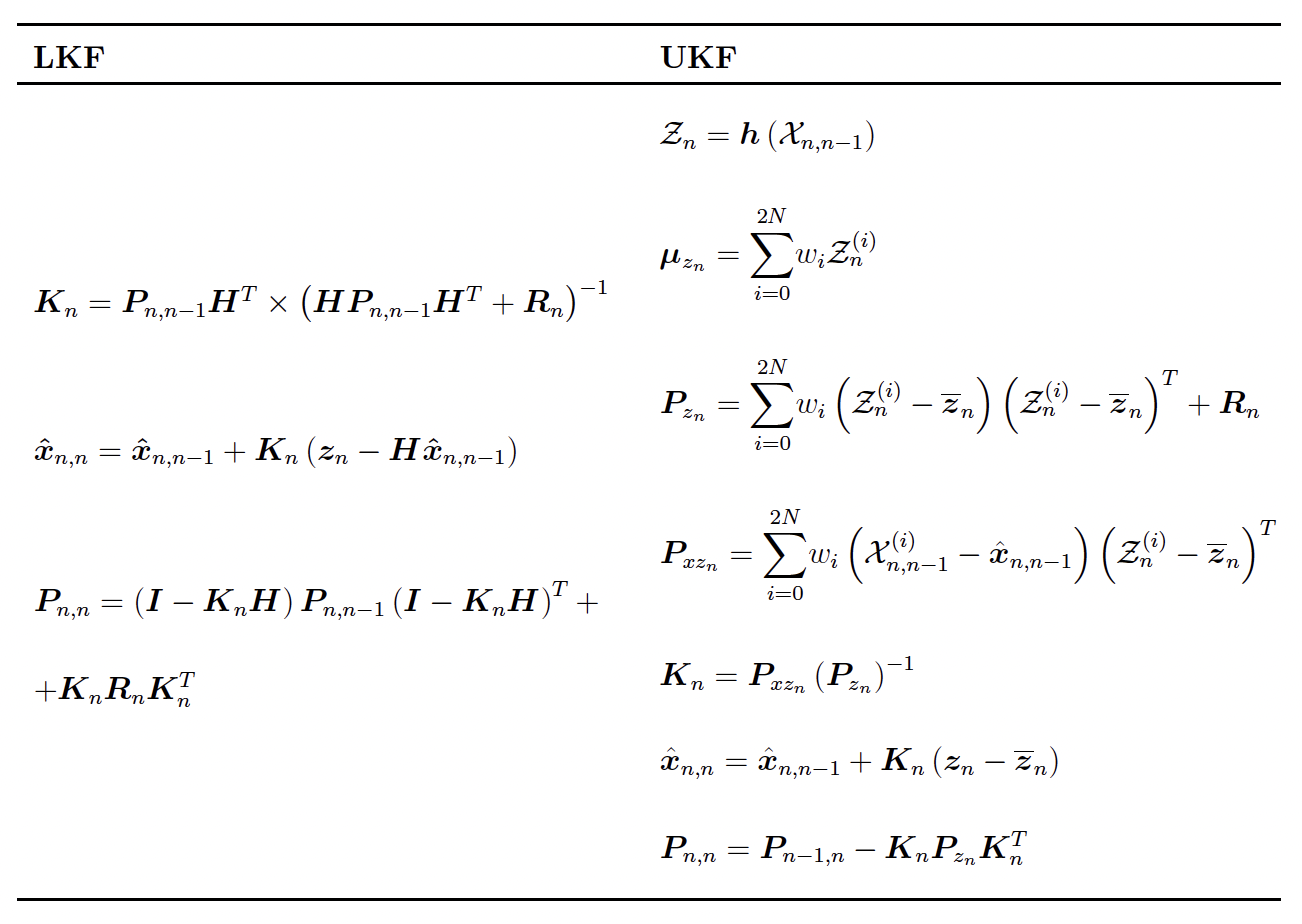
\includegraphics[width=0.9\linewidth]{Figures//Part3/UKF_UpdateSummary.png}
    \vspace{-12pt}
    \caption{LKF and UKF update stage equations.}
\end{figure}
\end{frame}

%%%%%%%%%%%%%%%%%%%%%%%%%%%%%%%%%%%%%%%%%%%%%%
\begin{frame}{The UKF algorithm Summary}
\begin{figure}
    \centering
    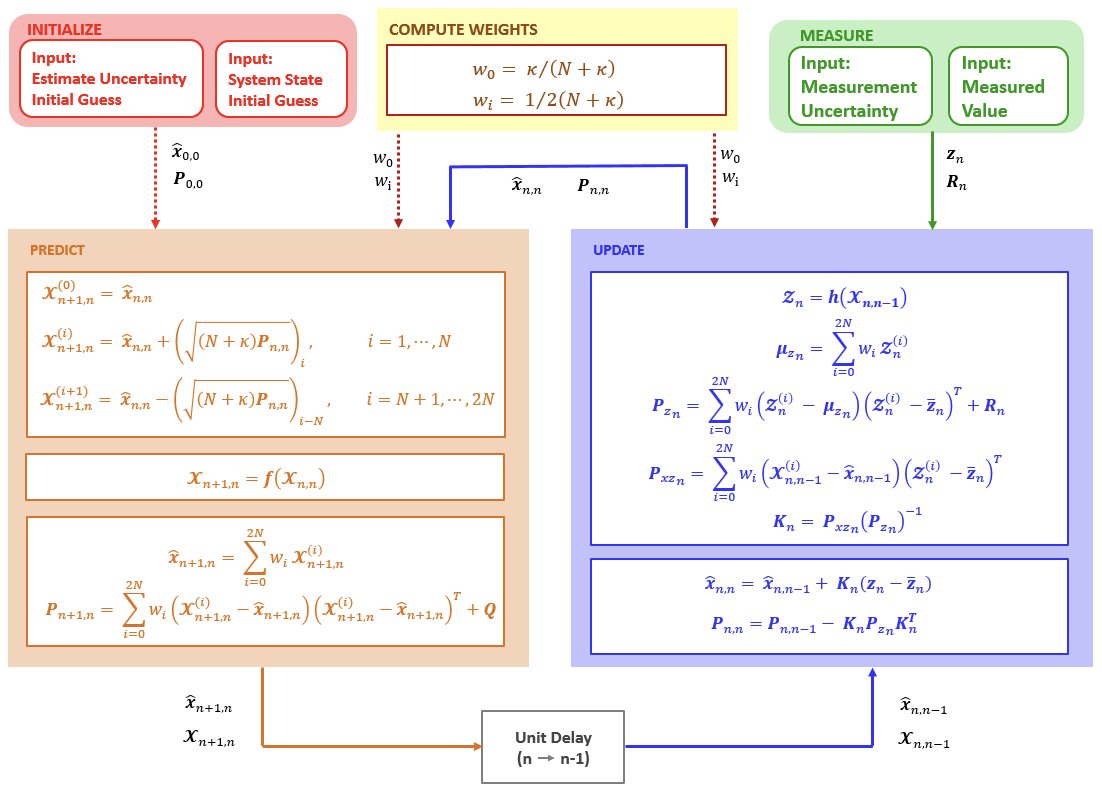
\includegraphics[width=0.85\linewidth]{Figures//Part3/UKFAlgorithmSummary.png}
    \caption{UKF algorithm summary diagram.}
\end{figure}
\end{frame}

%%%%%%%%%%%%%%%%%%%%%%%%%%%%%%%%%%%%%%%%%%%%%%
\subsubsection{Example 13 – vehicle location estimation using radar}
\begin{frame}{Example 13 – vehicle location estimation using radar}
Now we apply UKF to Example~11 (see Slide~\ref{Example11}).
\begin{columns}
        \column{0.5\textwidth} 
        \begin{itemize}
    \item We want to track the vehicle using radar, which is located at the plane origin, measuring the vehicle range ($r$) and the bearing angle ($\varphi$).
    \item The radar measurement error distribution is Gaussian. 
    \item The state transition matrix $\mathbf{F}$, the process noise matrix $\mathbf{Q}$, the measurement covariance
$\mathbf{R}$, and the measurement model $\mathbf{h}(\mathbf{x})$ are similar to example 11. 
\end{itemize}
\[
\mathbf{F} =
\begin{bmatrix}
1 & \Delta t & 0.5\Delta t^2 & 0 & 0 & 0 \\
0 & 1 & \Delta t & 0 & 0 & 0 \\
0 & 0 & 1 & 0 & 0 & 0 \\
0 & 0 & 0 & 1 & \Delta t & 0.5\Delta t^2 \\
0 & 0 & 0 & 0 & 1 & \Delta t \\
0 & 0 & 0 & 0 & 0 & 1
\end{bmatrix}
\]
        \column{0.5\textwidth}
        \[
\mathbf{Q} =
\begin{bmatrix}
\frac{\Delta t^4}{4} & \frac{\Delta t^3}{2} & \frac{\Delta t^2}{2} & 0 & 0 & 0 \\
\frac{\Delta t^3}{2} & \Delta t^2 & \Delta t & 0 & 0 & 0 \\
\frac{\Delta t^2}{2} & \Delta t & 1 & 0 & 0 & 0 \\
0 & 0 & 0 & \frac{\Delta t^4}{4} & \frac{\Delta t^3}{2} & \frac{\Delta t^2}{2} \\
0 & 0 & 0 & \frac{\Delta t^3}{2} & \Delta t^2 & \Delta t \\
0 & 0 & 0 & \frac{\Delta t^2}{2} & \Delta t & 1
\end{bmatrix}
\sigma^2_a
\]

\[
\mathbf{z}_n = \mathbf{h}(\mathbf{x}_n)
\]
\[
\mathbf{z}_n = 
\begin{bmatrix}
r \\
\phi
\end{bmatrix}
=
\begin{bmatrix}
\sqrt{x^2 + y^2} \\
\tan^{-1} \left(\frac{y}{x}\right)
\end{bmatrix}
\]

\[
\mathbf{R}_n =
\begin{bmatrix}
\sigma^2_{rm} & 0 \\
0 & \sigma^2_{\phi m}
\end{bmatrix}
=
\begin{bmatrix}
5^2 & 0 \\
0 & 0.0087^2
\end{bmatrix}
\]
\end{columns}    
\end{frame}

%%%%%%%%%%%%%%%%%%%%%%%%%%%%%%%%%%%%%%%%%%%%%%
\begin{frame}{Example 13 – vehicle location estimation using radar - Results}
\begin{columns}
        \column{0.4\textwidth}
        \vspace{-17pt}
\begin{figure}
    \centering
    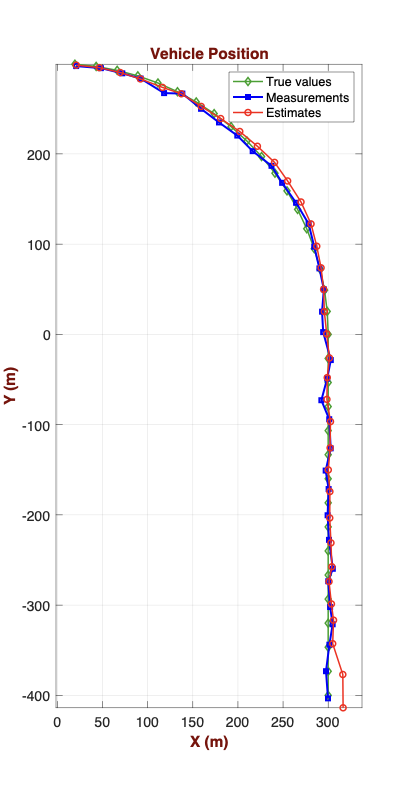
\includegraphics[width=0.7\linewidth]{Figures//Part3/Ex13_Position.png}
    %\caption{Enter Caption}
    \vspace{-17pt}
\end{figure}
    {\footnotesize Although the filter is roughly initiated at about 100 meters from the true position with zero initial velocity, it provides a good position estimation after taking two measurements and a velocity estimation after taking four measurements.}
        \column{0.6\textwidth}
        \vspace{-25pt}
        \begin{figure}
            \centering
            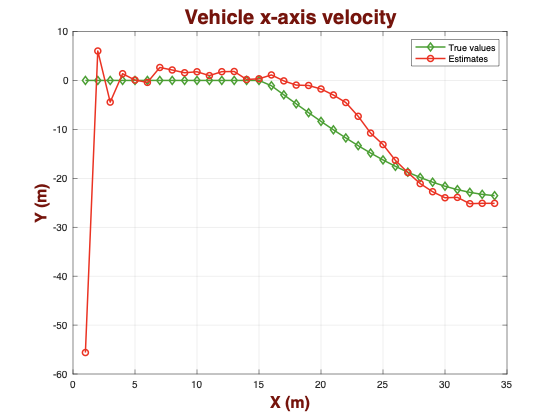
\includegraphics[width=0.7\linewidth]{Figures//Part3/Ex13_Vehicle_xVelocity.png}
            %\caption{Enter Caption}
        \end{figure}
        \vspace{-15pt}
        \begin{figure}
            \centering
            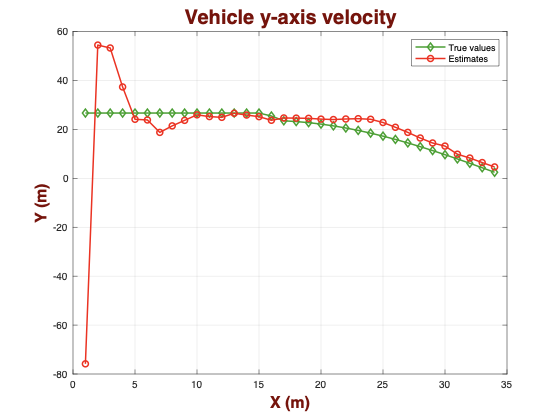
\includegraphics[width=0.7\linewidth]{Figures//Part3/Ex13_Vehicle_yVelocity.png}
            %\caption{Enter Caption}
        \end{figure}

        \texttt{\tiny [Code: Non-linear KF/Ex13\_UKF\_StatetoMeasurementUncertainty.m]}
        
\end{columns}    
\end{frame}

%%%%%%%%%%%%%%%%%%%%%%%%%%%%%%%%%%%%%%%%%%%%%%
\begin{frame}{Example 13 – vehicle location estimation using radar - Results}
\begin{columns}
        \column{0.5\textwidth} 
        \vspace{-10pt}
        \begin{figure}
            \centering
            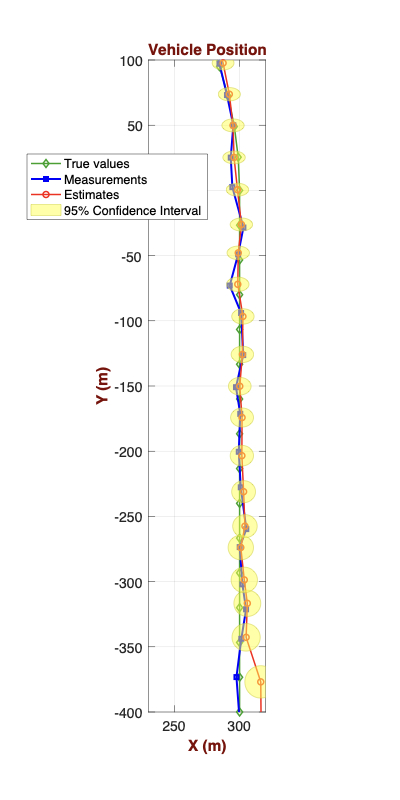
\includegraphics[trim={0 1.7cm 0 1.5cm},clip, width=0.6\linewidth]{Figures//Part3/Ex13_ZoomedPosition_StraightSegment.png}
        \end{figure}
        \begin{itemize}
            \item We can see that at the linear part of the vehicle motion, the UKF copes with the noisy measurements and follows the true vehicle position.
        \end{itemize}
            
        \column{0.5\textwidth}
        \vspace{-30pt}
        
        \begin{figure}
            \centering
            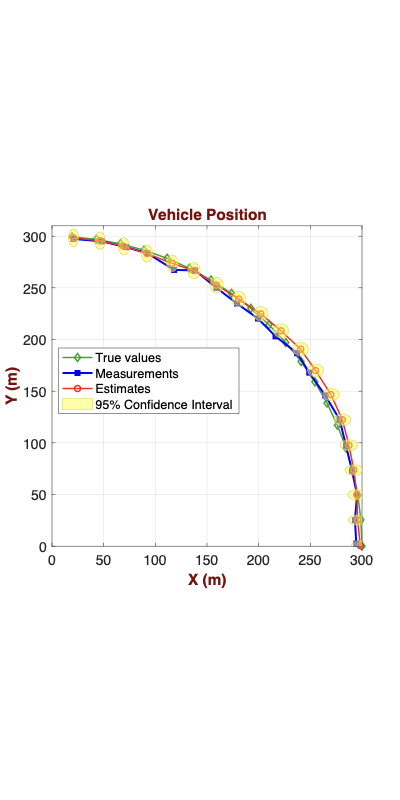
\includegraphics[trim={0 7cm 0 4cm},clip, width=0.8\linewidth]{Figures//Part3/Ex13_ZoomedPosition_CurvedSegment.png}
        \end{figure}
        \begin{itemize}            
            \item During the vehicle turning maneuver, the UKF estimates are quite away from the true vehicle position, although they are within the 90\% confidence ellipse bounds.
            \item We can see that the ellipses’ size constantly decreases. That means that the UKF converges with time.
        \end{itemize}
\end{columns}    
\end{frame}

%%%%%%%%%%%%%%%%%%%%%%%%%%%%%%%%%%%%%%%%%%%%%%
\subsubsection{Sigma Point Algorithm Modification}
\begin{frame}{Sigma Point Algorithm Modification}
\begin{columns}
        \column{0.5\textwidth} 
        \begin{itemize}
            \item The most common/accepted modification to the \textit{sigma point computation algorithm} in Unscented Transform is proposed in~\cite{Wan_SigmaPointModification_2000}.
            \item The algorithm parameterizes sigma point computation by $\alpha$, $\beta$, $\lambda$, and $\kappa$ tuning parameters. 
            \item The \textbf{first} key difference is the initial parameter $\lambda$ (i.e., $\kappa$ in UT) for the sigma points:
        
        \begin{equation*}
        \boxed{
        \lambda = \alpha^2 (N + \kappa) - N
        }
        \end{equation*}
        \vspace{-5pt}
        \begin{itemize}
            \item $N$ is the number of dimensions.
            \item $0<\alpha\leq 1$ determines the spread of the sigma points around the mean; usually set to a small positive value (e.g., $\alpha = 0.001$). Higher $\alpha \rightarrow$ higher spread. 
            \item $\kappa$ is a secondary scaling parameter that is usually set to 0.
            \item $\beta$ is used to incorporate prior knowledge of the distribution of the input random variable (for Gaussian distributions, $\beta = 2$ is optimal).
        \end{itemize}
        \end{itemize}
        \column{0.5\textwidth}
         \begin{itemize}
            \item Sigma points are calculated as before
            \item The \textbf{Second} difference is how the sigma oint weights are set:
            \begin{align*}
                w^{(m)}_0 &= \frac{\lambda}{N + \kappa} \\
                w^{(c)}_0 &= \frac{\lambda}{N + \lambda} + (1 - \alpha^2 + \beta) \\
                w_i &= \frac{1}{2(N + \lambda)}, \quad i > 0
                \end{align*}
                \begin{itemize}
                    \item $w^{(m)}_0$ is the weight for the first sigma point $\mathbf{\mathcal{X}}^{(0)}_{n,n}$ when computing the weighted mean.
                    \item $w^{(c)}_0$ is the weight for the first sigma point $\mathbf{\mathcal{X}}^{(0)}_{n,n}$ when computing the weighted covariance.
                    \item $w_i$ is the weight for the other sigma points $\mathbf{\mathcal{X}}^{(i)}_{n,n}$, $i > 0$ when computing the weighted mean or covariance.
                \end{itemize}
         \end{itemize}
\end{columns}    
\end{frame}

%%%%%%%%%%%%%%%%%%%%%%%%%%%%%%%%%%%%%%%%%%%%%%
\begin{frame}{Sigma Point Algorithm Modification}
\begin{columns}
        \column{0.5\textwidth}
        \begin{figure}
            \centering
            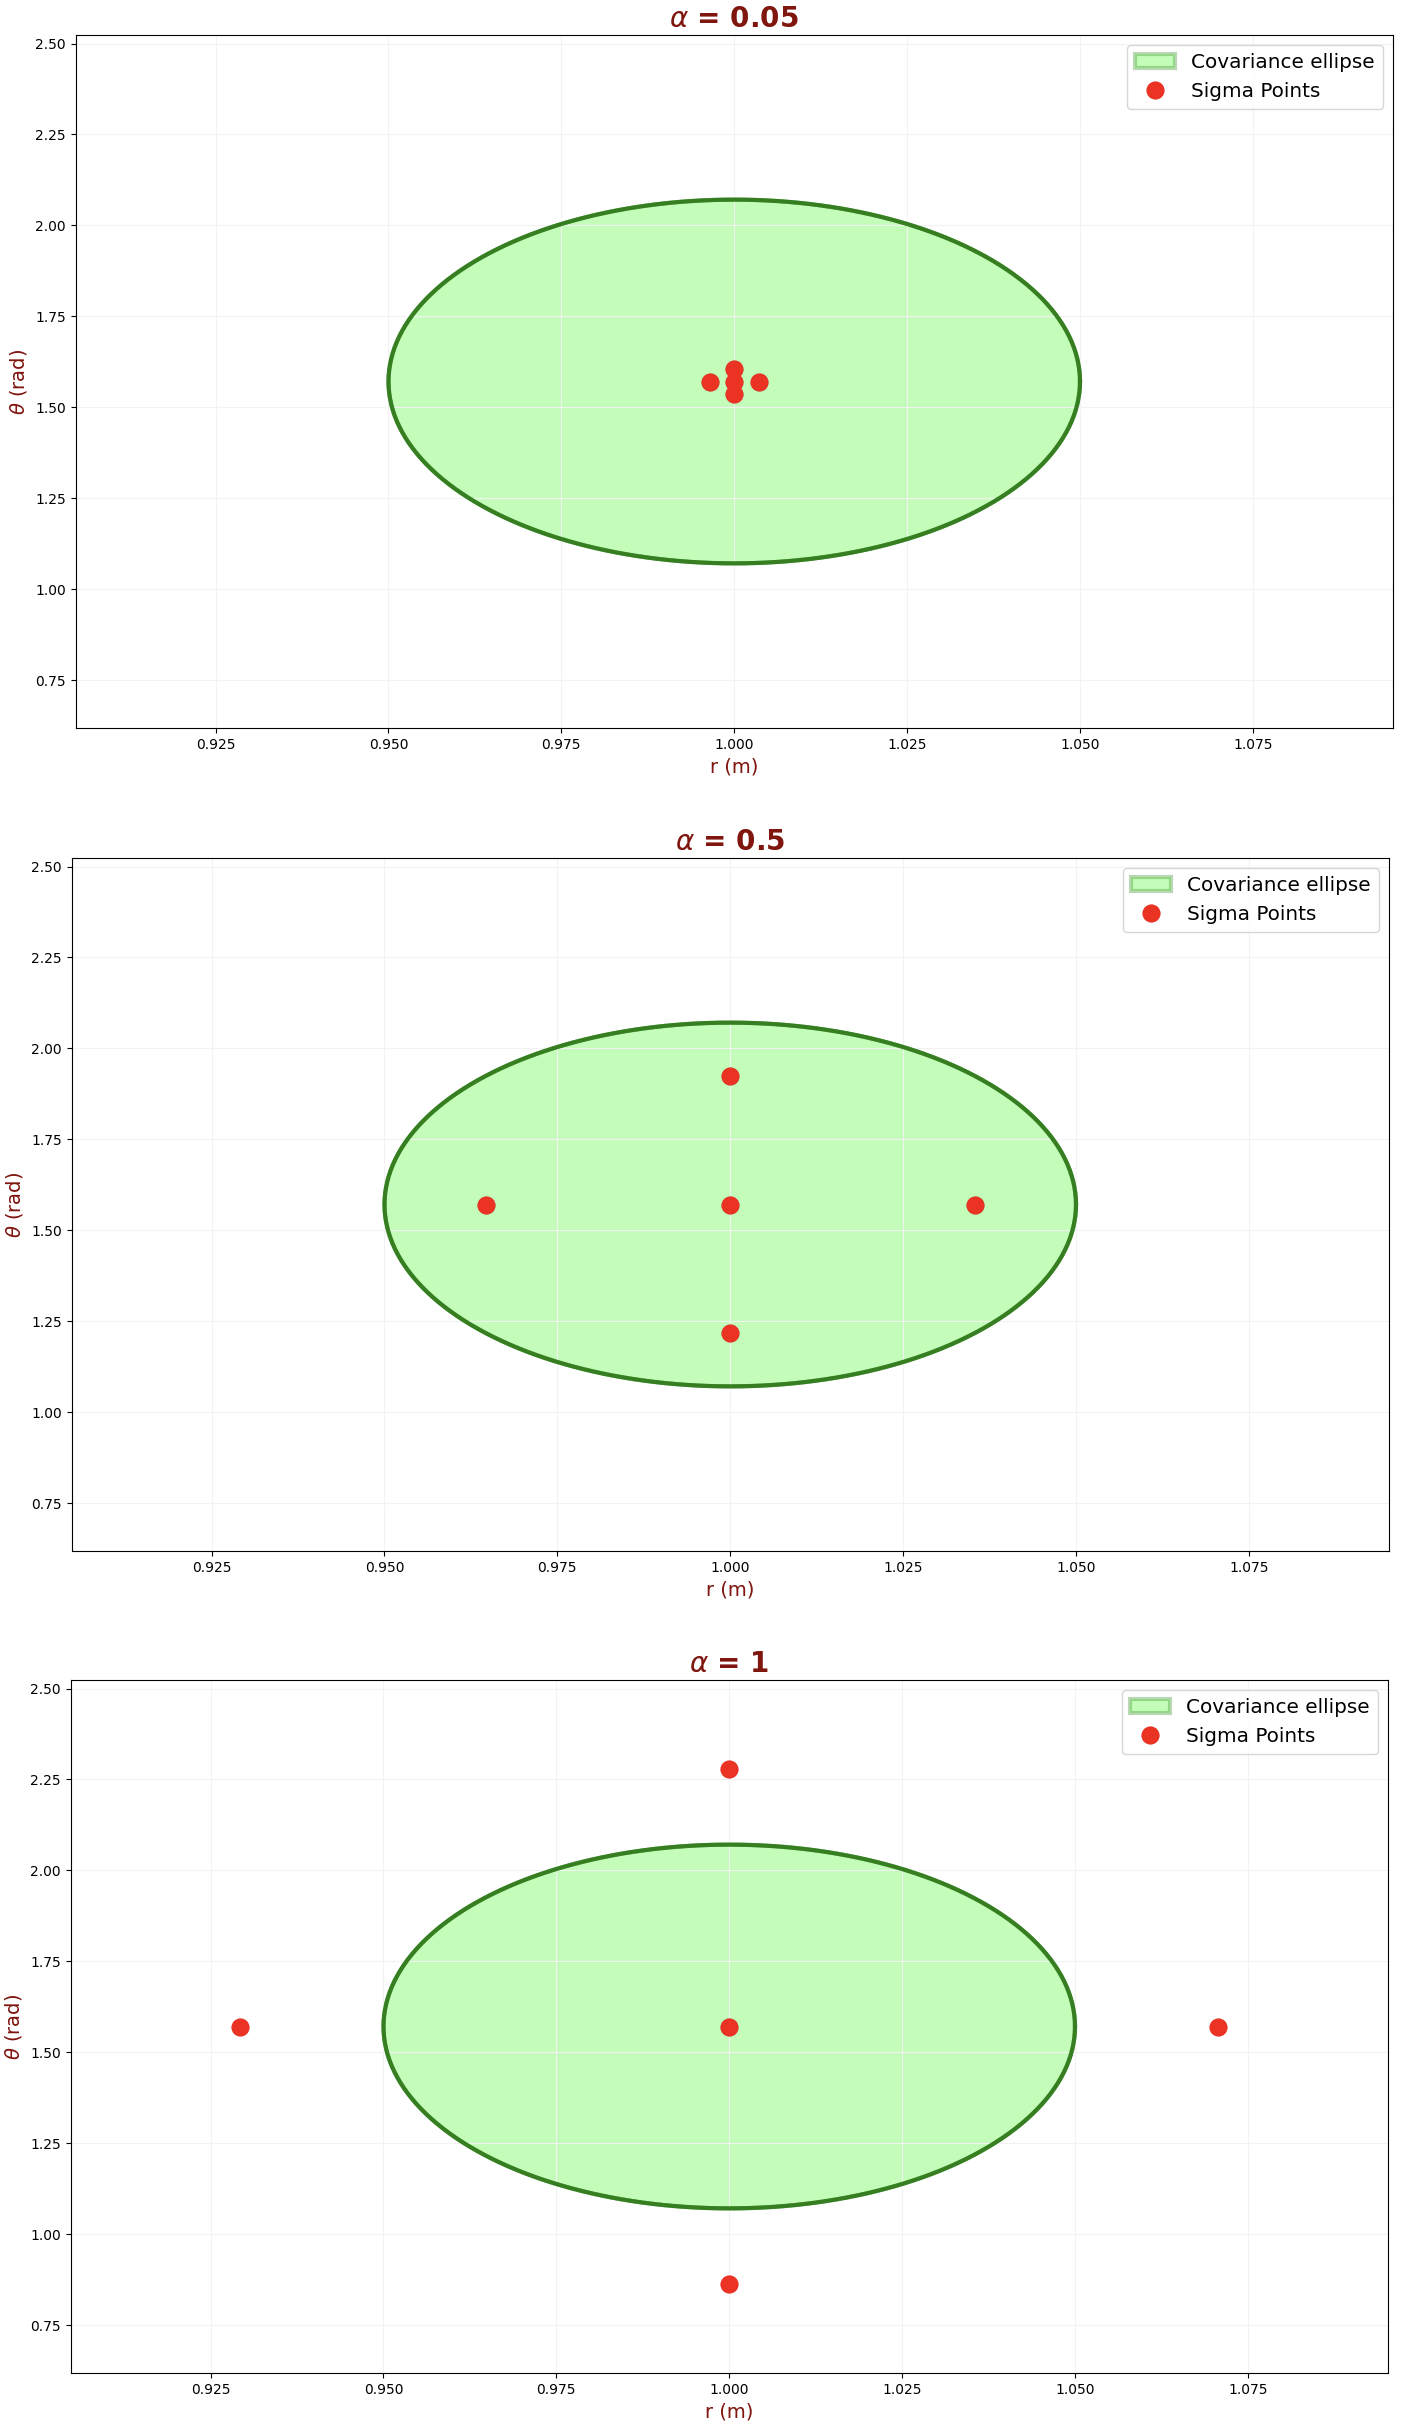
\includegraphics[trim={0 30cm 0 0cm},clip,, width=0.9\linewidth]{Figures//Part3/alphaEffectOnSigmaPoints.png}
            \caption{How $\alpha$ influences the Sigma Points.}
            %\vspace{-20pt}
        \end{figure}
        \column{0.5\textwidth}
        \begin{figure}
            \centering
            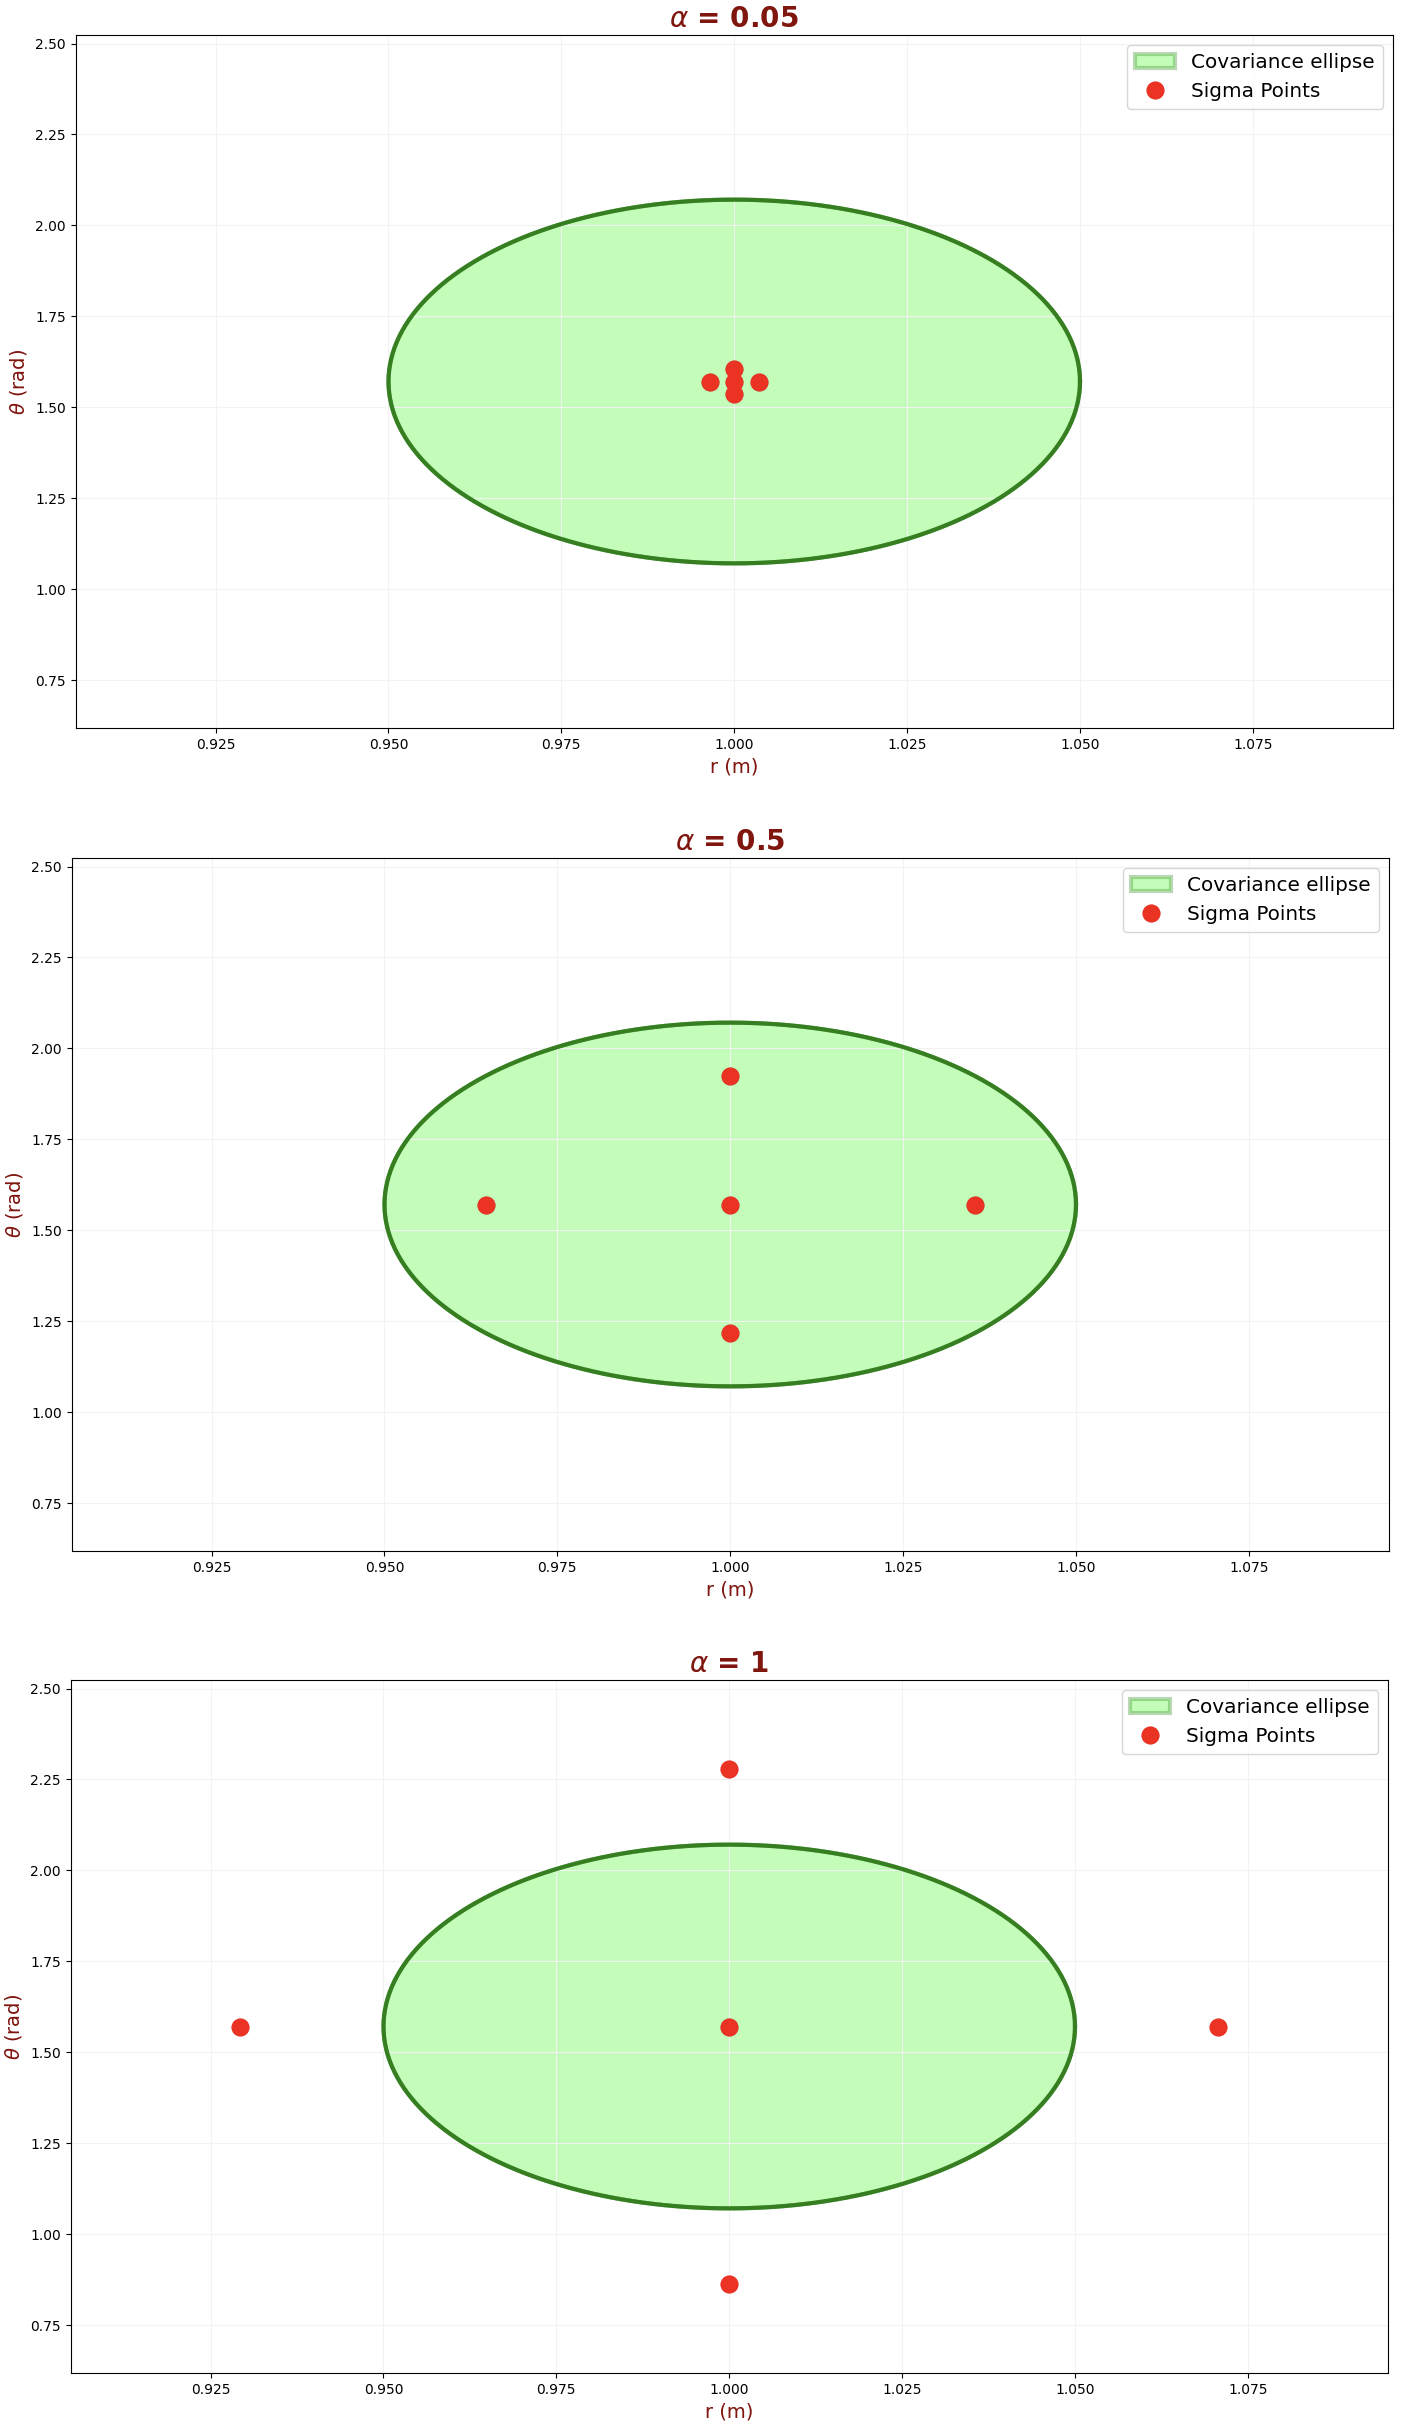
\includegraphics[trim={0 0cm 0 57cm},clip, width=0.9\linewidth]{Figures//Part3/alphaEffectOnSigmaPoints.png}
            \caption{How $\alpha$ influences the Sigma Points.}
            %\vspace{-20pt}
        \end{figure}

        \textcolor{blue}{One should experiment for the right choice of $\alpha$.}
\end{columns}    
\end{frame}

%%%%%%%%%%%%%%%%%%%%%%%%%%%%%%%%%%%%%%%%%%%%%%
\begin{frame}{Modified UKF algorithm summary}
  \begin{figure}
      \centering
      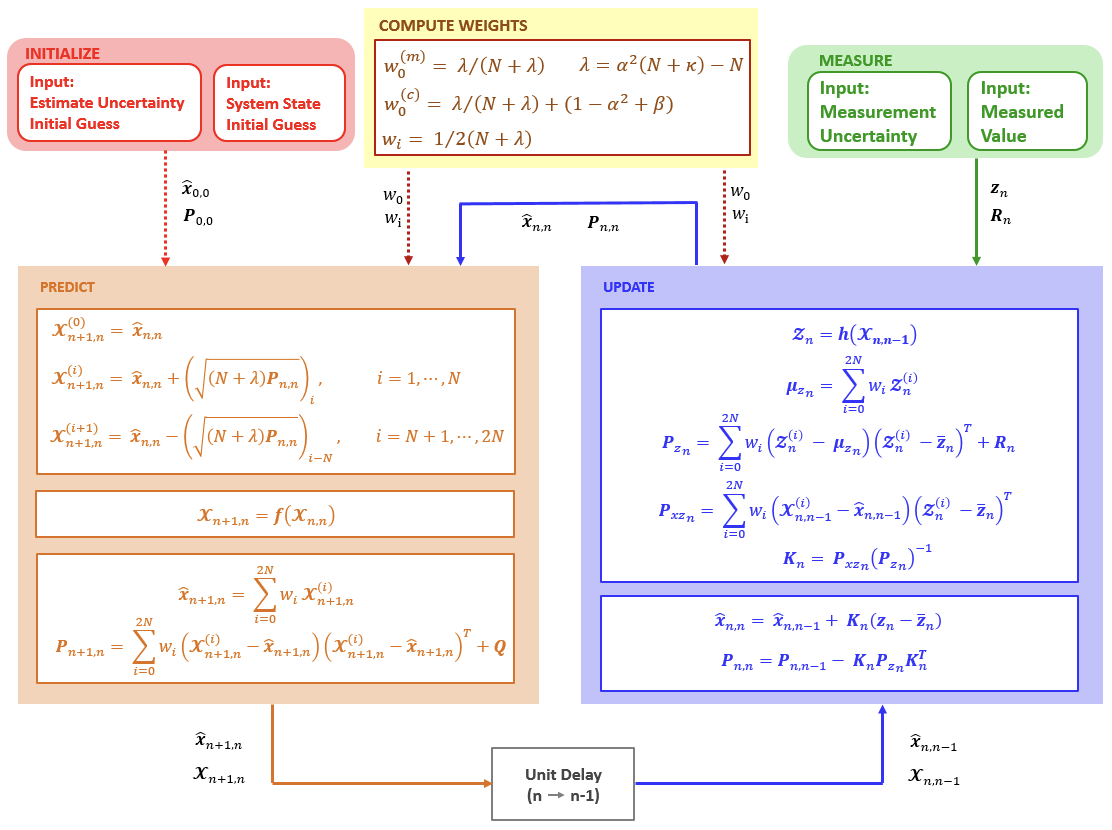
\includegraphics[width=0.85\linewidth]{Figures//Part3/Modified UKF Algorithm Summary.png}
      \caption{Modified UKF algorithm summary}
  \end{figure}
\end{frame}


%%%%%%%%%%%%%%%%%%%%%%%%%%%%%%%%%%%%%%%%%%%%%%
\subsubsection{Example 14 - Estimating the pendulum angle}
\begin{frame}{Example 14 - Estimating the pendulum angle}
\begin{columns}
\column{0.5\textwidth}
We measure the pendulum position $z = Lsin(\theta_n)$.

The state vector of the pendulum is:
\[
\mathbf{x}_n =
\begin{bmatrix}
\theta_n \\
\dot{\theta}_n
\end{bmatrix}
\]
where $\theta_n$ is the pendulum's angle  $\dot{\theta}_n$ the angular velocity at time $n$

The dynamic model of the pendulum is non-linear:
\[
\hat{\mathbf{x}}_{n+1,n} = \mathbf{f}(\hat{\mathbf{x}}_{n,n})
\]
\[
\hat{\mathbf{x}}_{n+1,n} =
\begin{bmatrix}
\hat{\theta}_{n+1,n} \\
\hat{\dot{\theta}}_{n+1,n}
\end{bmatrix}
=
\begin{bmatrix}
\hat{\theta}_{n,n} + \hat{\dot{\theta}}_{n,n} \Delta t \\
\hat{\dot{\theta}}_{n,n} - \frac{g}{L} \sin(\hat{\theta}_{n,n}) \Delta t
\end{bmatrix}
\]
\[
\mathbf{f}(\hat{\mathbf{x}}_{n,n}) =
\begin{bmatrix}
\hat{\theta}_{n,n} + \hat{\dot{\theta}}_{n,n} \Delta t \\
\hat{\dot{\theta}}_{n,n} - \frac{g}{L} \sin(\hat{\theta}_{n,n}) \Delta t
\end{bmatrix}
\]

The estimate covariance is:
\[
\mathbf{P} =
\begin{bmatrix}
p_{x} & p_{x\dot{x}} \\
p_{\dot{x}x} & p_{\dot{x}}
\end{bmatrix}
\]

\column{0.5\textwidth}
%\vspace*{-55pt}


The Process Noise Matrix:
\[
\mathbf{Q} =
\begin{bmatrix}
\sigma^2_{x} & \sigma^2_{x\dot{x}} \\
\sigma^2_{\dot{x}x} & \sigma^2_{\dot{x}}
\end{bmatrix}
=
\begin{bmatrix}
\frac{\Delta t^4}{4} & \frac{\Delta t^3}{2} \\
\frac{\Delta t^3}{2} & \Delta t^2
\end{bmatrix}
\sigma^2_{a}
\]
\textbf{The Measurement Equation}
We measure the pendulum position: $ z= L \sin(\theta_n)$, i.e., the state-to-measurement relation is non-linear:
\[
\mathbf{z}_n = \mathbf{h}(\mathbf{x}_n), \quad
\mathbf{h}(\mathbf{x}_n) = L \sin(\theta_n)
\]

\textbf{The Measurement Uncertainty} is:
\[
\mathbf{R}_n =
\begin{bmatrix}
\sigma^2_{x_m}
\end{bmatrix}
\]
\end{columns}   
\end{frame}

%%%%%%%%%%%%%%%%%%%%%%%%%%%%%%%%%%%%%%%%%%%%%%
\begin{frame}{Example 14 - Estimating the pendulum angle}
\begin{columns}
        \column{0.5\textwidth} 
        \begin{figure}
            \centering
            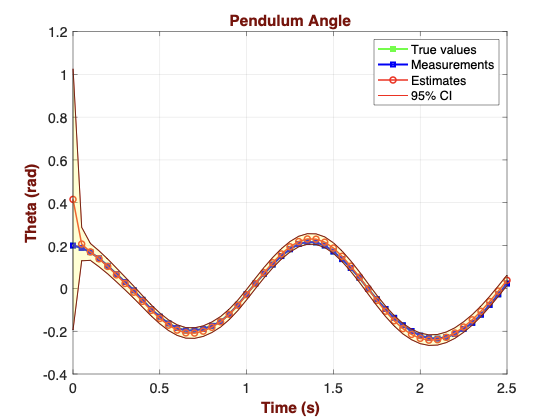
\includegraphics[width=0.9\linewidth]{Figures//Part3/Ex14_PendulumAngle_modifiedUKF.png}
        \end{figure}
        \column{0.5\textwidth}
        \begin{figure}
            \centering
            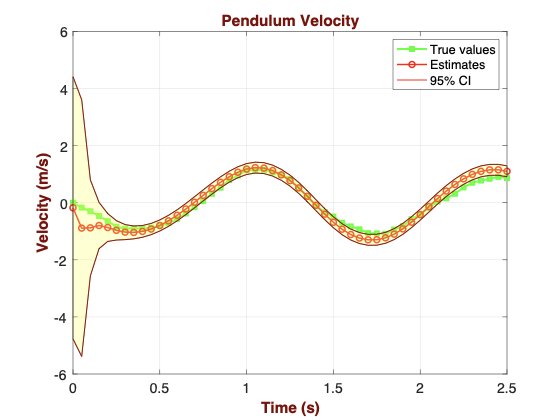
\includegraphics[width=0.9\linewidth]{Figures//Part3/Ex14_PendulumVelocity_ModifiedUKF.png}
        \end{figure}
\end{columns} 

        \texttt{\tiny [Code: Non-linear KF/Ex14\_UKF\_for\_Estimating\_PendulumAngle.m]}
\end{frame}

%%%%%%%%%%%%%%%%%%%%%%%%%%%%%%%%%%%%%%%%%%%%%%
\begin{frame}{Example 14 - Estimating the pendulum angle}
The results without the original UKF are as follows. There seems to be less uncertainty in pendulum angles estimates compared to the modified-UKF results. 
\begin{columns}
        \column{0.5\textwidth} 
        \begin{figure}
            \centering
            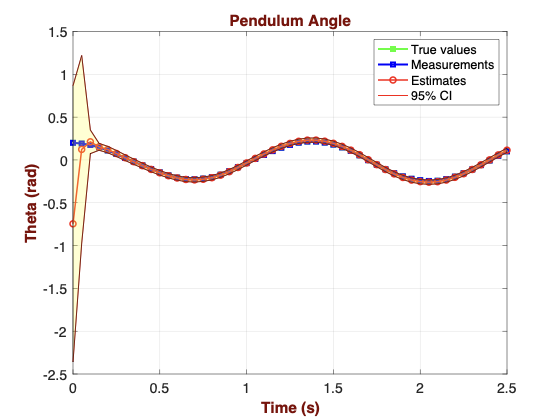
\includegraphics[width=0.9\linewidth]{Figures//Part3/Ex14_PendulumAngle_UKF.png}
        \end{figure}
        \column{0.5\textwidth}
        \begin{figure}
            \centering
            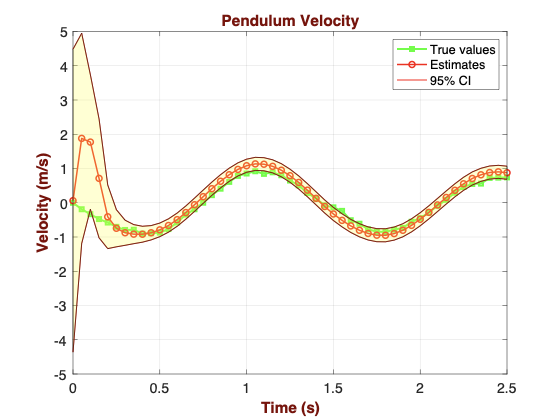
\includegraphics[width=0.9\linewidth]{Figures//Part3/Ex14_PendulumVelocity_UKF.png}
        \end{figure}
\end{columns}    
\end{frame}

%%%%%%%%%%%%%%%%%%%%%%%%%%%%%%%%%%%%%%%%%%%%%%
\subsubsection{Non-linear filters comparison: EKF vs UKF}
\begin{frame}{Non-linear filters comparison: EKF vs UKF}
Example 11 (EKF) and Example 13 (UKF) dealt with vehicle location estimation using radar. Both examples have identical parameters: vehicle dynamics, radar, initialization, and measurements. \texttt{\tiny{[Code:Non-linear KF/EKFvsUKF\_VehileTrackingExamples.m]}}

\begin{columns}
        \column{0.5\textwidth} 
        \begin{figure}
            \centering
            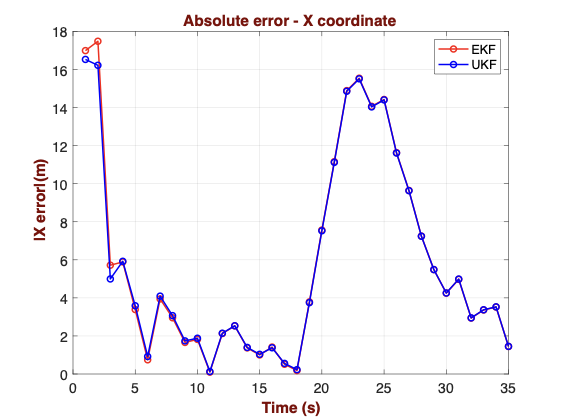
\includegraphics[width=0.6\linewidth]{Figures//Part3/EKFvsUKF_Error_Xcoord.png}
        \end{figure}
        \vspace{-10pt}
        \begin{figure}
            \centering
            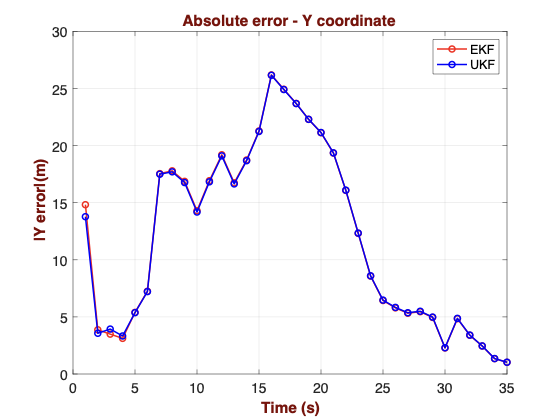
\includegraphics[width=0.6\linewidth]{Figures//Part3/EKFvsUKF_Error_Ycoord.png}
        \end{figure}
        UKF performs slightly better for the first two iterations, but then the filters converge, and the performance of becomes identical.
        \column{0.5\textwidth}
        \begin{figure}
            \centering
            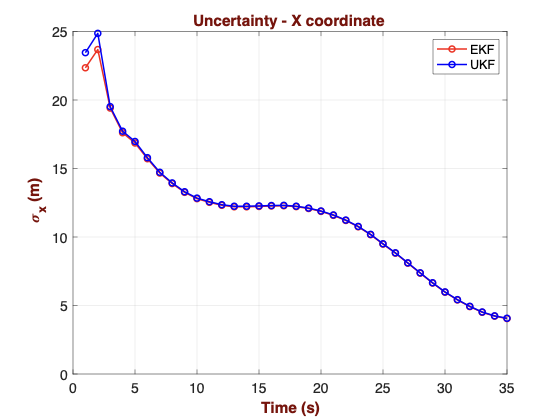
\includegraphics[width=0.6\linewidth]{Figures//Part3/EKFvsUKF_Uncertainty_Xcoord.png}
        \end{figure}
        \vspace{-10pt}
        \begin{figure}
            \centering
            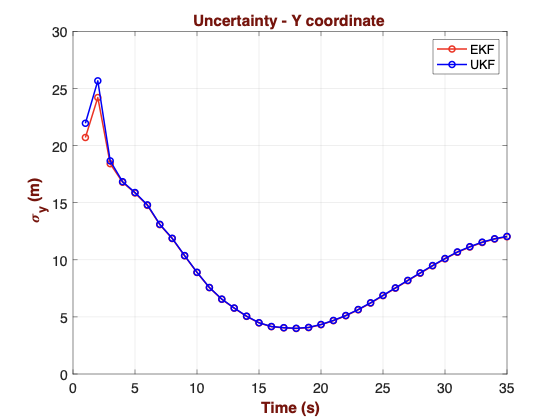
\includegraphics[width=0.6\linewidth]{Figures//Part3/EKFvsUKF_Uncertainty_Ycoord.png}
        \end{figure}
        The estimation uncertainties are also identical for both filters.
\end{columns}    
\end{frame}
%%%%%%%%%%%%%%%%%%%%%%%%%%%%%%%%%%%%%%%%%%%%%%
\begin{frame}{Example 14 - estimating the pendulum angle}
Example 12 (EKF) and Example 14 (UKF) dealt the estimation of the pendulum angle and angular
velocity. Both examples have identical parameters: pendulum dynamics, initialization, and measurements. \texttt{\tiny{[Code: Non-linear KF/EKFvsUKF\_PendulumExamples.m]}}
\begin{columns}
        \column{0.5\textwidth}
        \begin{figure}
            \centering
            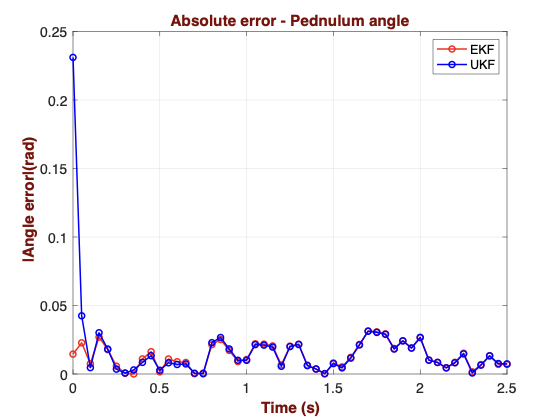
\includegraphics[width=0.6\linewidth]{Figures//Part3/EKFvsUKF_AE_PendulumAngle.png}
        \end{figure}
        \vspace{-10pt}
        \begin{figure}
            \centering
            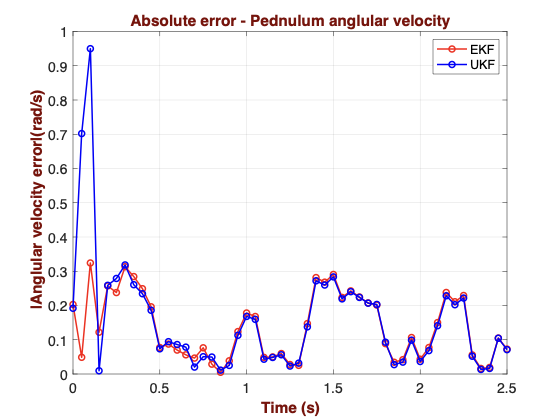
\includegraphics[width=0.6\linewidth]{Figures//Part3/EKFvsUKF_AE_PendulumAVelocity.png}
        \end{figure}
        During the first 0.5 seconds, the UKF error is significantly higher.
        \column{0.5\textwidth}
        \begin{figure}
            \centering
            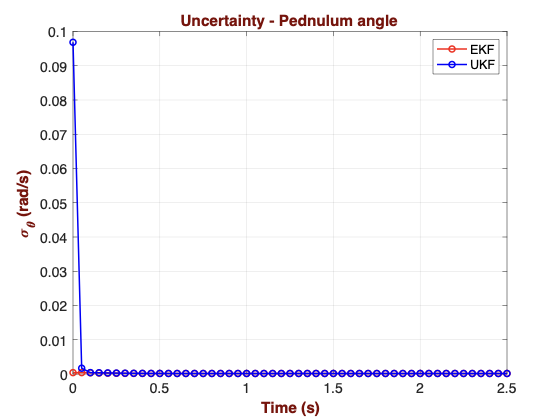
\includegraphics[width=0.6\linewidth]{Figures//Part3/EKFvsUKF_Uncertainty_PendulumAngle.png}
        \end{figure}
        \vspace{-10pt}
        \begin{figure}
            \centering
            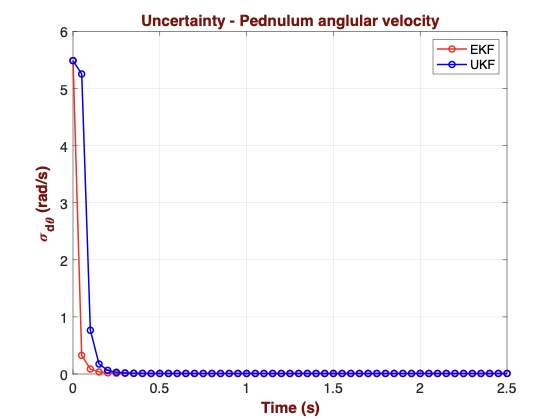
\includegraphics[width=0.6\linewidth]{Figures//Part3/EKFvsUKF_Uncertainty_PendulumAVelocity.png}
        \end{figure}
        During the filter convergence period, the UKF uncertainty is higher than the EKF uncertainty.
\end{columns}    
\end{frame}

%%%%%%%%%%%%%%%%%%%%%%%%%%%%%%%%%%%%%%%%%%%%%%

%%%%%%%%%%%%%%%%%%%%%%%%%%%%%%%%%%%%%%%%%%%%%%
\begin{frame}{Conclusions}
\begin{itemize}
    \item Extended and Unscented Kalman Filters perform a \textbf{linear approximation of the
dynamic and state-to-measurement models}.

\item The Extended Kalman Filter is a standard and most common technique used in
non-linear estimation problems. Although the EKF became a standard for non-linear
estimation, almost 60 years of EKF usage experience has led to a consensus that it is
\textbf{unreliable for highly non-linear models}.

    \item The UKF is considered to be a better choice compared to EKF as demonstrated by examples in the original work~\cite{julier1997new} and \cite{van2004sigma}.
\item In the vehicle location examples, we have seen a similar performance of UKF and EKF. In the pendulum measurement example, the UKF was
even better during the filter convergence period.

\item Since both filters are sub-optimal, it is  recommended testing both filters, and then choosing a better approach.

\item \textcolor{blue}{\textbf{Particle Filter:}} The particle filter uses
using \textcolor{blue}{Monte-Carlo method} technique for approximation. It is considered a precise
technique; however, it often requires thousands of times more computations. One can find a good tutorial in \cite{elfring2021particle}, along with the code.
\end{itemize}
\end{frame}


